% concatenated from main-23.tex
%%%%% section{Preamble}
\documentclass[12 pt]{amsart}
% --c \documentclass[11pt,letterpaper,oneside]{amsart}
  \usepackage[utf8]{inputenc}
  \usepackage[margin=3cm]{geometry}
  \setlength{\textheight}{21cm}
  \setlength{\textwidth}{15cm}  
  
%\usepackage{titletoc, tocloft}
%\setlength{\cftsubsecindent}{1cm}
%\setlength{\cftsubsubsecindent}{2cm}
%\dottedcontents{section}[1.5em]{}{1.3em}{.6em}


\setcounter{tocdepth}{1}
\makeatletter
\def\l@subsection{\@tocline{1}{0pt}{2pc}{1pc}{}}
\def\l@subsubsection{\@tocline{2}{0pt}{2pc}{1pc}{}}
\makeatother

  %subsection{Packages}
  \usepackage{stmaryrd}
\usepackage{amsmath,amssymb,amsthm, mathrsfs, mathtools, bbold, mathbbol}
\usepackage{amscd,mathtools}
\usepackage{comment}
  \usepackage{geometry}
  \usepackage{graphicx,epstopdf}
  \usepackage{color,xcolor}
  \usepackage{enumerate}
  \usepackage{xspace}
  \usepackage{tipa}
  \usepackage[user,titleref]{zref}
%  \usepackage{showlabels}
 \usepackage{soul}
 \usepackage{xcolor}
  %\usepackage{amscd}
 % \usepackage[notcite,notref]{showkeys}
  \usepackage{epsfig}
 % \usepackage{pinlabel}
 % \usepackage[all]{xy}
  
\usepackage{tikz}
\usetikzlibrary{shapes.geometric}
\usetikzlibrary{angles}


\usepackage{caption, subcaption}
\usepackage{tikz-cd}
\usetikzlibrary{calc,decorations.pathreplacing}
\usepackage{tikz}
\usetikzlibrary{calc}
\usetikzlibrary{arrows}
\usetikzlibrary{decorations.pathreplacing}
\usetikzlibrary{intersections}
\usepackage{xcolor}
\usepackage{xspace}
\usepackage{todonotes}


%\usepackage[dvips]{graphicx}
%\usepackage{color}              % Need the color package
%\usepackage{epsfig}
%
%\usepackage{tikz}
%\usetikzlibrary{calc,through,backgrounds, arrows}
%\usetikzlibrary{decorations.pathmorphing, decorations.pathreplacing,positioning,fit}. 
%

\usepackage{mathrsfs}
\usetikzlibrary{matrix}
\usetikzlibrary{positioning}
\DeclareMathAlphabet{\pazocal}{OMS}{zplm}{m}{n}
% set arrows as stealth fighter jets
\tikzset{>=stealth}
  %\usepackage{color}
  %\definecolor{darkgreen}{rgb}{0, 0.40, 0}

  %\usepackage{amsthm} %%% Defines \theoremstyle
  %\usepackage{amsmath} %%% Defines \numberwithin, \operatorname
  %\usepackage{amssymb} %%% Defines \mathbb

  %\usepackage{psfrag}

  \usepackage{hyperref}

  \hypersetup{
    colorlinks=true,
    linkcolor=blue,
    filecolor=magenta,      
    urlcolor=cyan,
    citecolor=purple,
    pdftitle={Overleaf Example},
    pdfpagemode=FullScreen,
    }

\usepackage{float}


  %%%%% subsection{Fonts} 

  %% Calligraphy 

  \newcommand{\calA}{\mathcal{A}}
  \newcommand{\calB}{\mathcal{B}}
  \newcommand{\calC}{\mathcal{C}}
  \newcommand{\calD}{\mathcal{D}}
  \newcommand{\calE}{\mathcal{E}}
  \newcommand{\calF}{\mathcal{F}}
  \newcommand{\calG}{\mathcal{G}}
  \newcommand{\calH}{\mathcal{H}}
  \newcommand{\calI}{\mathcal{I}}
  \newcommand{\calJ}{\mathcal{J}}
  \newcommand{\calK}{\mathcal{K}}
  \newcommand{\calL}{\mathcal{L}}
  \newcommand{\calM}{\mathcal{M}}
  \newcommand{\calN}{\mathcal{N}}
  \newcommand{\calO}{\mathcal{O}}
  \newcommand{\calP}{\mathcal{P}}
  \newcommand{\calQ}{\mathcal{Q}}
  \newcommand{\calR}{\mathcal{R}}
  \newcommand{\calS}{\mathcal{S}}
  \newcommand{\calT}{\mathcal{T}}
  \newcommand{\calU}{\mathcal{U}}
    \newcommand{\calV}{\mathcal{V}}
  \newcommand{\calW}{\mathcal{W}}
  \newcommand{\calX}{\mathcal{X}}
  \newcommand{\calY}{\mathcal{Y}}
  \newcommand{\calZ}{\mathcal{Z}}
  
  %%%%this paper
  

  

    \newcommand{\Uout}{ \calU_{\rm \, Out}}
    \newcommand{\pin}{\partial_{\rm \, In} }
    \newcommand{\pout}{\partial_{\rm Out}} 
  \newcommand{\Rin}{R^{\rm in}}

  %% Math Bold

  \renewcommand{\AA}{\mathbb{A}}
  \newcommand{\BB}{\mathbb{B}}
  \newcommand{\CC}{\mathbb{C}}
  \newcommand{\DD}{\mathbb{D}}
  \newcommand{\EE}{\mathbb{E}}
  \newcommand{\FF}{\mathbb{F}}
  \newcommand{\HH}{\mathbb{H}}
  \newcommand{\KK}{\mathbb{K}}
  \newcommand{\MM}{\mathbb{M}}
  \newcommand{\NN}{\mathbb{N}}
  \newcommand{\OO}{\mathbb{O}} 
  \newcommand{\PP}{\mathbb{P}}
  \newcommand{\QQ}{\mathbb{Q}}
  \newcommand{\RR}{\mathbb{R}}
  \renewcommand{\SS}{\mathbb{S}}
  \newcommand{\TT}{\mathbb{T}}
  \newcommand{\VV}{\mathbb{V}}
  \newcommand{\WW}{\mathbb{W}}
  \newcommand{\XX}{\mathbb{X}}
  \newcommand{\YY}{\mathbb{Y}}
  \newcommand{\ZZ}{\mathbb{Z}}

  %% Text bold
  
  \newcommand{\bfa}{\textbf{a}}
  \newcommand{\bfb}{\textbf{b}}
  \newcommand{\bfc}{\textbf{c}}  
  \newcommand{\bfd}{\textbf{d}} 
  \newcommand{\bfx}{\textbf{x}}  
  \newcommand{\bfz}{\textbf{z}}  

  %% Gothic letters
  
  \newcommand{\gothic}{\mathfrak}
  \newcommand{\Ga}{{\gothic a}}
  \newcommand{\Gb}{{\gothic b}}
  \newcommand{\Gc}{{\gothic c}}
  \newcommand{\Gd}{{\gothic d}}
  \newcommand{\Ge}{{\gothic e}}
  \newcommand{\Gf}{{\gothic f}}
  \newcommand{\GF}{{\gothic F}}
  \newcommand{\Gg}{{\gothic g}}
  \newcommand{\Gh}{{\gothic h}}
  \newcommand{\Gi}{{\gothic i}}
  \newcommand{\Gj}{{\gothic j}}
  \newcommand{\Gk}{{\gothic k}}
  \newcommand{\Gl}{{\gothic l}}
  \newcommand{\Gm}{{\gothic m}}
  \newcommand{\gn}{{\gothic n}}
  \newcommand{\go}{{\gothic o}}
  \newcommand{\Gp}{{\gothic p}}
  \newcommand{\Gq}{{\gothic q}}
  \newcommand{\Gr}{{\gothic r}}
  \newcommand{\Gs}{{\gothic s}}
  \newcommand{\Gt}{{\gothic t}}
  \newcommand{\Gu}{{\gothic u}}
  \newcommand{\gv}{{\gothic v}}
  \newcommand{\Gw}{{\gothic w}}
  \newcommand{\gx}{{\gothic x}}
  \newcommand{\gy}{{\gothic y}}
  \newcommand{\Gz}{{\gothic z}}
  \newcommand{\GS}{{\gothic S}}
  

\newcommand{\rE} {{\mathcal{E} }}
\newcommand{\rEB} {{\mathcal{EB} }}

  %%%%%% subsection{Standard Math}

  %% Environments and Numbering 

  \newtheorem{theorem}{Theorem}[section]
  \newtheorem{proposition}[theorem]{Proposition}
  \newtheorem{corollary}[theorem]{Corollary}
  \newtheorem{lemma}[theorem]{Lemma}
  \newtheorem{conjecture}[theorem]{Conjecture}
  \newtheorem{problem}[theorem]{Problem}
  \newtheorem{question}[theorem]{Question}
  \newtheorem{claim}[theorem]{Claim}
  \newtheorem{subclaim}[theorem]{Subclaim}
  \newtheorem*{claim*}{Claim}

  \newtheorem{introthm}{Theorem}
  \newtheorem{introcor}[introthm]{Corollary}
  \newtheorem{introprop}[introthm]{Proposition} 
  \newtheorem{introques}[introthm]{Question} 
  \renewcommand{\theintrothm}{\Alph{introthm}}
  \renewcommand{\theintrocor}{\Alph{introcor}}
  \renewcommand{\theintroprop}{\Alph{introprop}}
  \renewcommand{\theintroques}{\Alph{introques}}

  \theoremstyle{definition}
  \newtheorem{definition}[theorem]{Definition}

  \newtheorem{exercise}[theorem]{Exercise}
  \newtheorem{example}[theorem]{Example}
  \newtheorem{fact}[theorem]{Fact}
  \newtheorem*{question*}{Question}
  \newtheorem*{answer*}{Answer}
  \newtheorem*{application*}{Application}
  \newtheorem{notation}[theorem]{Notation}

  \theoremstyle{remark}
  \newtheorem{remark}[theorem]{Remark}
  \newtheorem*{remark*}{Remark}
  
%  \numberwithin{equation}{section}

  %% References

  \newcommand{\secref}[1]{Section~\ref{#1}}
  \newcommand{\thmref}[1]{Theorem~\ref{#1}}
  \newcommand{\corref}[1]{Corollary~\ref{#1}}
  \newcommand{\lemref}[1]{Lemma~\ref{#1}}
  \newcommand{\propref}[1]{Proposition~\ref{#1}}
  \newcommand{\clmref}[1]{Claim~\ref{#1}}
  \newcommand{\remref}[1]{Remark~\ref{#1}}
  \newcommand{\exaref}[1]{Example~\ref{#1}}
  \newcommand{\facref}[1]{Fact~\ref{#1}}
  \newcommand{\exref}[1]{Exercise~\ref{#1}}
  \newcommand{\figref}[1]{Figure~\ref{#1}}
  \newcommand{\defref}[1]{Definition~\ref{#1}}
  \newcommand{\probref}[1]{Problem~\ref{#1}}
  \newcommand{\eqnref}[1]{Equation~\eqref{#1}}
  \newcommand{\mf}[1]{\mathfrak{#1}}
  \newcommand{\fo}{{\mathfrak{o}}}
  \newcommand{\opi}{{\overline \pi}}
    \newcommand{\oX}{{\overline X}}

  %% Operators:

  \DeclareMathOperator{\Mod}{Mod}
    \DeclareMathOperator{\Sat}{Sat}
  \DeclareMathOperator{\Ext}{Ext}
  \DeclareMathOperator{\Hyp}{Hyp}
  \DeclareMathOperator{\special subset}{special subset}
  \DeclareMathOperator{\area}{area}
  \DeclareMathOperator{\I}{i}
  \DeclareMathOperator{\Vol}{Vol}
  \DeclareMathOperator{\Area}{Area}
  \DeclareMathOperator{\twist}{twist}
  \DeclareMathOperator{\tw}{tw}
  \DeclareMathOperator{\fold}{fold}
  \DeclareMathOperator{\green}{stretch}

  %% Inequalities:

  \newcommand{\emul}{\stackrel{{}_\ast}{\asymp}}
  \newcommand{\gmul}{\stackrel{{}_\ast}{\succ}}
  \newcommand{\lmul}{\stackrel{{}_\ast}{\prec}}
  \newcommand{\eadd}{\stackrel{{}_+}{\asymp}}
  \newcommand{\gadd}{\stackrel{{}_+}{\succ}}
  \newcommand{\ladd}{\stackrel{{}_+}{\prec}}

  %% Relations

  \newcommand{\isotopic}{\mathrel{\approx}}
  \newcommand{\homeo}{\mathrel{\cong}} % Homeomorphism
  \newcommand{\nhomeo}{\mathrel{\not\cong}}
  \newcommand{\isom}{\cong} % Isomorphism
  \newcommand{\disjoint}{\mathbin{\amalg}} % Disjointness
  \newcommand{\cross}{\times}
  \newcommand{\cutby}{\mathbin{\rule[.023 in]{.12 in}{.02 in}}} 
  \newcommand{\derivative}[2]{ \frac{{\partial{#1}}{\partial{#2}} } }
  \newcommand{\pka}{\partial_{\kappa}}
  % \newcommand{\ps}{\partial_s}
  \newcommand{\kp}{\kappa^{\rm path}}

  %% Spaces

  \newcommand{\Aut}{\ensuremath{\operatorname{Aut}}\xspace} 
       % Automorphism group
 % \newcommand{\Out}{\ensuremath{\operatorname{Out}}\xspace} 
       % Outer automorphism group
  \newcommand{\Inn}{\ensuremath{\operatorname{Inn}}\xspace} 
      % Inner automorphism group

   \newcommand{\GL}{\ensuremath{\operatorname{GL}}\xspace} 
       % General linear
  \newcommand{\SL}{\ensuremath{\operatorname{SL}}\xspace} 
       % Special linear
  \newcommand{\PGL}{\ensuremath{\operatorname{PGL}}\xspace} 
         % Projective general linear
  \newcommand{\PSL}{\ensuremath{\operatorname{PSL}}\xspace} 
       % Projective special linear
  \newcommand{\SO}{\ensuremath{\operatorname{SO}}\xspace} 
       % Special orthogonal

  \newcommand{\Map}{\ensuremath{\operatorname{Map}}\xspace}  
  \newcommand{\MCG}{\ensuremath{\mathcal{MCG}}\xspace}  
       % Mapping class group
  \newcommand{\AC}{\ensuremath{\mathcal{AC}}\xspace} 
       % Arc and Curve Complex

  \newcommand{\T}{\ensuremath{\mathcal{T}}\xspace} 
       % Teichmuller space
  \newcommand{\MF}{\ensuremath{\mathcal{MF}}\xspace} 
       % Measured foliations
  \newcommand{\PMF}{\ensuremath{\mathcal{PMF}}\xspace} 
       % Projectively measured foliations
  \newcommand{\ML}{\ensuremath{\mathcal{ML}}\xspace} 
         % Ditto for laminations
  \newcommand{\FL}{\ensuremath{\mathcal{FL}}\xspace} 
       % Filling laminations
  \newcommand{\EL}{\ensuremath{\mathcal{EL}}\xspace} 
        % Ending laminations
  \newcommand{\PML}{\ensuremath{\mathcal{PML}}\xspace}  
        % Projectivised measured laminations

  \newcommand{\Mark}{\ensuremath{\mathcal{MK}}\xspace}  
        % Marking graph

  %% Constants

  \newcommand{\sA}{{\sf A}}   
  \newcommand{\sB}{{\sf B}}   
  \newcommand{\sC}{{\sf C}}   
  \newcommand{\sD}{{\sf D}}     
  \newcommand{\sE}{{\sf E}}   
  \newcommand{\sF}{{\sf F}}   
  \newcommand{\sG}{{\sf G}}   
  \newcommand{\sH}{{\sf H}}     
  \newcommand{\sI}{{\sf I}}   
  \newcommand{\sJ}{{\sf J}}   
 \newcommand{\sK}{{\sf K}}   
  \newcommand{\sL}{{\sf L}}     
  \newcommand{\sM}{{\sf M}}   
  \newcommand{\sN}{{\sf N}}   
  \newcommand{\sO}{{\sf O}}   
  \newcommand{\sP}{{\sf P}}       
  \newcommand{\sQ}{{\sf Q}}   
  \newcommand{\sR}{{\sf R}}   
  \newcommand{\sS}{{\sf S}}     
  \newcommand{\sT}{{\sf T}}   
  \newcommand{\sU}{{\sf U}}   
  \newcommand{\sV}{{\sf V}}   
  \newcommand{\sW}{{\sf W}}     
  \newcommand{\sX}{{\sf X}}   
  \newcommand{\sY}{{\sf Y}}   
  \newcommand{\sZ}{{\sf Z}}     
  
  
  \renewcommand{\bfa}{{\sf a}}   
   \renewcommand{\bfd}{{\sf d}}  

  \newcommand{\bb}{{\sf b}}   
  \newcommand{\cc}{{\sf c}}   
  \newcommand{\dd}{{\sf d}}     
  \newcommand{\ee}{{\sf e}}   
  \newcommand{\ff}{{\sf f}}   
  %\renewcommand{\gg}{{\sf g}}   
  \newcommand{\hh}{{\sf h}}     
  \newcommand{\ii}{{\sf Ii}}   
  \newcommand{\jj}{{\sf j}}   
  \newcommand{\kk}{{\sf k}}   
  \renewcommand{\ll}{{\sf l}}     
  \newcommand{\mm}{{\sf m}}   
  \newcommand{\nn}{{\sf n}}   
  \newcommand{\oo}{{\sf o}}   
  \newcommand{\pp}{{\sf p}}       
  \newcommand{\qq}{{\sf q}}   
  \newcommand{\rr}{{\sf r}}   
  \renewcommand{\ss}{{\sf s}}     
  \renewcommand{\tt}{{\sf t}}   
  \newcommand{\uu}{{\sf u}}   
  \newcommand{\vv}{{\sf v}}   
  \newcommand{\ww}{{\sf w}}     
  \newcommand{\xx}{{\sf x}}   
  \newcommand{\yy}{{\sf y}}   
  \newcommand{\zz}{{\sf z}}   
      
  \newcommand{\radius}{{\sf r}}


%% Distances 

  \newcommand{\dL}{{d_L}} 
  \newcommand{\dT}{{d_T}} 
  \newcommand{\dS}{{d_S}} 


  %% Bars

  \newcommand{\balpha}{{\overline \alpha}}
  \newcommand{\bbeta}{{\overline \beta}}
  \newcommand{\bgamma}{{\overline \gamma}}
  \newcommand{\bphi}{{\overline \phi}}  
  \newcommand{\bnu}{{\overline \nu}}    
  \newcommand{\ba}{{\overline a}}
  \newcommand{\bc}{{\overline c}}
  \newcommand{\bd}{{\overline d}}  
  \newcommand{\be}{{\overline e}}
  \renewcommand{\bf}{{\overline f}}
  \newcommand{\bk}{{\overline k}}  
  \newcommand{\bp}{{\overline p}}
  \newcommand{\bq}{{\overline q}}
  \newcommand{\bx}{{\overline x}}
   \newcommand{\by}{{\overline y}}
   \newcommand{\bz}{{\overline z}}
   \newcommand{\bw}{{\overline w}}
   \newcommand{\bG}{{\overline \calG}}          
   \newcommand{\bI}{{\overline I}}  
   \newcommand{\oG}{{\overline \Gamma}}
   \newcommand{\eventual}{{\stackrel{e}{=}}}


  \newcommand{\ua}{{\underline a}}
  \newcommand{\ub}{{\underline b}}
  \newcommand{\uc}{{\underline c}}
    \newcommand{\oC}{{\overline C}}
  \newcommand{\supp}{{\rm supp}}
  \newcommand{\pf}{{\partial_{\rm f}}}
    \newcommand{\ps}{{\partial_s}}
  \newcommand{\pQ}{{\partial_{\rm f} Q}}

  %% Others:
\DeclareMathOperator{\Core}{Core}
\DeclareMathOperator{\Outer}{CV}
\DeclareMathOperator{\out}{Out}
\DeclareMathOperator{\diam}{diam}
\DeclareMathOperator{\Cay}{Cay}
\DeclareMathOperator{\Pen}{Pen}
\DeclareMathOperator{\C}{C}
\DeclareMathOperator{\deep}{deep}
\DeclareMathOperator{\trans}{trans}



\newcommand{\CV}{{\Outer_{\! n}}}
\newcommand{\Out}{\out(\F)}
 
\newcommand{\CAT}{\ensuremath{\operatorname{CAT}(0)}\xspace}      

%% Long Words  

  \newcommand{\Teich}{{Teichm\"uller }} % A Nazi dude
  \hyphenation{geo-desics} 
  \newcommand{\Ham}{{Hamenst\"adt }}


  %------
  % Don't mess with this unless you know what you're doing.
  % (It creates a squarish vertically centered dot that can be used to
  %  indicate a free parameter.)
    
  \newcommand{\param}{{\mathchoice{\mkern1mu\mbox{\raise2.2pt\hbox{$
  \centerdot$}}
  \mkern1mu}{\mkern1mu\mbox{\raise2.2pt\hbox{$\centerdot$}}\mkern1mu}{
  \mkern1.5mu\centerdot\mkern1.5mu}{\mkern1.5mu\centerdot\mkern1.5mu}}}
  %------

\DeclarePairedDelimiterX{\norm}[1]{\lvert}{\rvert}{#1}
\DeclarePairedDelimiterX{\Norm}[1]{\lVert}{\rVert}{#1}

  \renewcommand{\setminus}{{\smallsetminus}}
  \renewcommand{\th}{{\rm th}}
%  \newcommand{\st}{\mathbin{\mid}} 
  \newcommand{\ST}{\mathbin{\Big|}} 
  \newcommand{\from}{\colon\thinspace} 
  \newcommand{\ep}{\epsilon}
  \newcommand{\bdy}{\partial} 
  \newcommand{\vis}{\bdy_\infty}
  \newcommand{\F}{{\FF_n}} 
  \newcommand{\ra}{{\rightarrow}}
  %\newcommand{\A}{{A(\Gamma)}}
  \newcommand{\ga}{{\gamma}}
  \newcommand{\bdf}{{\partial_{f} }}
 \newcommand{\pc}{{ \partial_{c} }}
 \newcommand{\hG}{{\hat{G}}}
  \newcommand{\hu}{{\hat{u}}}
    \newcommand{\hv}{{\hat{v}}}
      \newcommand{\hw}{{\hat{w}}}
 
 \newcommand\tab[1][1cm]{\hspace*{#1}}
\newcommand{\cat}[1]{{\mathscr{#1}}}
\newcommand{\D}{\delta}
\newcommand{\R}{\mathbb{R}}
\newcommand{\A}{\alpha}
\newcommand{\B}{\beta}
\newcommand{\p}{\partial}
\newcommand{\K}{\kappa}
\newcommand{\n}{\eta}
\newcommand{\hd}{\hat{d}}
\newcommand{\hX}{\widehat{X}}

\newcommand{\ob}{\mathfrak{o}}

%\newcommand{\CAT}{\ensuremath{\operatorname{CAT}(0)}\xspace}         
    
%  \newcommand{\CV}{{\Outer_{\! }}}
%  \DeclareMathOperator{\out}{Out}
%   \newcommand{\Out}{\out(\F)}  

\newcommand{\myGlobalTransformation}[2]
{
    \pgftransformcm{1}{0}{0.5}{0.3}{\pgfpoint{#1}{#2}}
}

    
%  \newcommand{\param}{{\mathchoice{\mkern1mu\mbox{\raise2.2pt\hbox{$
%  \centerdot$}}
%  \mkern1mu}{\mkern1mu\mbox{\raise2.2pt\hbox{$\centerdot$}}\mkern1mu}{
%  \mkern1.5mu\centerdot\mkern1.5mu}{\mkern1.5mu\centerdot\mkern1.5mu}}}
%  %------


   
    
%\newcommand{\ps}{\partial_{s}}
  
\newcommand{\Ccom}[1]{\Cmod\marginpar{\color{red}\tiny #1 --gt}} 
\newcommand{\Cmod}{$\textcolor{red}{\clubsuit}$} 

\newcommand{\Kcom}[1]{\Kmod\marginpar{\color{black}\tiny #1 --kr}} 
\newcommand{\Kmod}{$\textcolor{black}{\clubsuit}$} 

\newcommand{\Ycom}[1]{\Ymod\marginpar{\color{blue}\tiny #1 --yq}} 
\newcommand{\Ymod}{$\textcolor{blue}{\clubsuit}$} 

%%%%%%%%%%%%%%%%%%%preamble added by Yulan ends here
\title[First passage percolation preserves sublinearly Morse boundaries]{First passage percolation preserves sublinearly Morse boundaries}
\author{Sagnik Jana}
 \address{Department of Mathematics,  University of Tennessee at Knoxville, Knoxville, TN, USA}
\email{sjana1@vols.utk.edu}

 
  \author{Yulan Qing}
 %\thanks{grants}
 \address{Department of Mathematics,  University of Tennessee at Knoxville, Knoxville, TN, USA}
 \email{yqing@utk.edu}
 


\begin{document}
\maketitle
\begin{abstract}
Sublinearly Morse directions in proper geodesic spaces are defined by sublinearly Morse stability. In this paper we offer an alternative  characterization for sublinearly Morse geodesic lines via middle recurrence. We then study first passage percolation (FPP) on proper geodesic graphs of bounded degree. We associate an i.i.d. collection of random passage times to each edge. Under suitable conditions on the passage time distribution,  we prove that sublinearly Morse boundaries are invariant under first passage percolation.
\end{abstract}

\section{Introduction}
 A sublinearly Morse boundary \cite{QRT1,QRT2} is a topological space consists of quasi-geodesic rays in a given metric space. It is constructed to extend the Gromov boundary beyond the hyperbolic setting. If the metric space in question, denoted $X$, is proper and geodesic, then the sublinearly Morse boundary, denoted $\ps X$,  is always quasi-isometrically invariant and metrizable. In many situations $\ps X$ provides a natural group-invariant topological model compatible with probabilistic boundary theory for random walks on $X$. A closely related topological set, the Morse boundary \cite{Cordes,CS} of metric spaces is often non-metrizable and does not always realize the Poisson boundary. These distinctions make the sublinearly Morse boundary particularly well-suited for studying asymptotic geometry alongside stochastic and dynamical phenomena. It is natural to ask how sublinearly Morse directions behave under random perturbations of the geometry. One natural model for such perturbations is first passage percolation (FPP), which systematically introduce randomness to graphs. In this process, one assigns i.i.d.\ random weights to the edges, and then defines the distance between two vertices as the smallest total weight among all paths joining them. The path that achieves this minimum is called a geodesic (an optimal path)[see section \ref{fpp}]. For the Cayley graph of $\mathbb{Z}^2$ with respect to the standard generators, this model was introduced by Hammersley and Welsh \cite{HW65}. While first passage percolations on $\mathbb{Z}^2$ and, more generally, on $\mathbb{Z}^d$ has been studied extensively and proven to be hard. For instance, it is still unknown whether bi-infinite geodesics exist (see \cite{Kesten}) after first passage percolation on $\mathbb{Z}^2$. Much less is known for other metric spaces until recently. Existence of bi-infinite geodesics and other interesting results \cite{BZ12,BT17} were obtained when the graph is Gromov hyperbolic.
 
Indeed, \cite{BT17} shows that if $X$ contains a bi-infinite Morse geodesic line, then $X_\omega$ contains a bi-infinite geodesic line almost surely. However, one surprise is that  \cite{BJQ} demonstrates that FPP does not, in general, preserve the Morseness of geodesic lines (a property all geodesic lines in hyperbolic spaces enjoy). This motivates the authors of this paper to study the problem in a setting that contains more hyperbolic behavior than $\ZZ^d$ but less than that of a hyperbolic graph. Specifically, we are interested in understand what happends to \emph{sublinear Morse} directions: recently \cite{JanaQing1} establishes that if $X$ has a bi-infinite sublinearly Morse geodesic line, then $X_\omega$ contains a bi-infinite geodesic line almost surely. Therefore, the immediate motivating question for this paper is:
\begin{question}
Are sublinearly Morseness of sets almost surely preserved under first  passage percolations? 
\end{question}



% First passage percolation is a process that can be modeled as random perturbation of metric on a given metric graph. In this paper, we shall restrict to the simplest model, where random i.i.d. lengths are assigned to the edges of a fixed combinatorial graph. 

% Let us briefly recall how first passage percolation is defined. We consider a connected non-oriented graph $X$, whose set of vertices (resp. edges) is denoted by $V$ (resp. E). For every function $\omega: E \rightarrow(0, \infty)$, we equip $V$ with the weighted graph metric $d_{\omega}$, where each edge $e$ has weight $\omega(e)$. In other words, for every $v_{1}, v_{2} \in V, d_{\omega}\left(v_{1}, v_{2}\right)$ is defined as the infimum over all path $\gamma=\left(e_{1}, \ldots, e_{m}\right)$ joining $v_{1}$ to $v_{2}$ of $|\gamma|_{\omega}:=\sum_{i=1}^{m} \omega\left(e_{i}\right)$. Observe that the graph metric on $V$ corresponds to the case where $\omega$ is constant equal to 1 , we shall simply denote it by $d$. We will now consider a probability measure on the set of all weight functions $\omega$. We let $\nu$ be a probability measure supported on $[0, \infty)$. Our model consists in choosing independently at random the weights $\omega(e)$ according to $\nu$. More formally, we equip the space $\Omega=[0, \infty)^{E}$ with the product probability that we denote by $P$.

% A famous open problem in percolation theory is whether with positive probability, first passage percolation on $\mathbb{Z}^{2}$ admits a bi-infinite geodesic. In his Saint-Flour course from 84 ', Kesten attributes this question to Furstenberg (see \cite{Keston}). Licea and Newman[??] made partial progress on this problem, which is still open, and mentioned that the conjecture that there are no such geodesics arose independently in the physics community studying spin glass. Wehr and Woo [16] proved absence of two sided infinite geodesic in a half plane, assuming the lengths distribution is continuously distributed with a finite mean. 
% The picture spaces with some negaive curvature is drastically different. In \cite{BT17} it is established that if $X$ has a bi-infinite Morse geoddesic line, then $X_\omega$ contains a bi-infinite geodesic line almost surely. However, in \cite{BJQ1} it is shown that first passage percolation do not preserve the Morseness of geodesic lines. Naturally we consider weaker notions of Morse: sublinearly Morse. In \cite{JanaQing1} it is established that  if $X$ has a bi-infinite \emph{sublinearly Morse} geodesic line, then $X_\omega$ contains a bi-infinite geodesic line almost surely. Therefore, the immediate motivating question for this project is:
% \begin{question}
% Are sublinearly Morseness of sets almost surely preserved under first  passage percolations? 
% \end{question}
We answer the question positively:
\begin{introthm}\label{introthm1}
Let $X$ be a graph with uniformly bounded degree and $\p_s X \neq \emptyset$.  Assume that the edge length distribution has finite expectation and also $\nu(\{0\}) = 0$. Then let $\omega$ be induced graphs with weight functions. Then for almost every $\omega$, such the first passage percolation induces a homeomorphism on the sublinearly Morse boundaries: $\p_s X \simeq \p_s X_\omega$.
\end{introthm}

This result opens up the possibility of analysis into the interaction between sublinearly Morse sets and first passage percolations. We give several natural and immediate questions that can be investigated.
%Let us first introduce some notation. Let $X$ be a simple graph, with no double edges. Recall that a path $\gamma=\left(e_{1}, \ldots, e_{n}\right)$ between two vertices $x, y$ is a sequence of consecutive edges joining $x$ to $y$. We denote $(x=\gamma(0), \ldots, \gamma(n)=y)$ the set of vertices such that for all $0 \leq i<n, \gamma(i)$ and $\gamma(i+1)$ are joined by the edge $e_{i+1}$. For all $i<j$, we shall also denote by $\gamma([i, j])$ the subpath $\left(e_{i+1}, \ldots, e_{j}\right)$ joining $\gamma(i)$ to $\gamma(j)$. Similarly, we define infinite paths indexed by $\mathbb{N}$ (resp. bi-infinite paths indexed by $\mathbb{Z}$).

Since first passage percolation does not preserve quasi-geodesics, this paper depends on characterizations of sublinear Morseness using paths of bounded slope. This notion is established for Morse geodesic rays and is utilized  in \cite{DMS} and improved in \cite{ADT}. We first develop an proper analogue of such a notion in the context of sublinear Morseness:
\begin{definition} \label{def:middle recurrent}
We say that a path (geodesic line or quasi-geodesic) $\gamma$ is \emph{middle third recurrent} if for every $C\geq1$ there is a constant $c$ (depends on $C$ and $\gamma$) such that the following holds: 
    for any path $p$ with endpoints $a,b \in \gamma$ satisfying $\ell(p)\leq Cd(a,b)$, intersects the $c\cdot \kappa$-neighborhood of the middle third of $\gamma[a,b]$ for some sublinear function $\kappa$. That is,
\[ p \cap \calN_{\kappa} (\gamma_{\frac 13[a,b]}, c )\neq \emptyset.\]
Where, $\gamma_{\frac{1}{3}[a,b]} := \biggl\{x\in \gamma : \min \{d(x,a),d(x,b)\} \ge \frac{1}{3}\cdot d(a,b)\biggr\}$.
\end{definition}
We are able to establish the path characterization of sublinearly Morse sets:

\begin{introthm}\label{introthm2}
A geodesic ray is sublinearly Morse if and only if it has the middle third recurrent property.

\end{introthm}

We remark that it is communicated to the authors during the preparation of this document that one of the directions of this characterization, Proposition 3.4, is also in the process of being established by Raghunath
Jaganathan Vennila as part of his research project. 


%\begin{introthm}\label{introthm2}
%Let $G$ be a finitely generated group where $\pka G \neq \emptyset$. $X$ be the Cayley graph of $G$ with respect to the generating set. Assume on the edge length distribution, $\EE \omega_e < \infty$ and $\nu(\{0\}) = 0$. Then for almost every $\omega$, $\pka G$ is invariant under first passage percolation.
%\end{introthm}

\begin{comment}
\subsection*{History}
For the Cayley graph of $\ZZ^2$ with respect to standard generators, first passage percolation was introduced by Hammersley and Welsh \cite{HW65} more than fifty years back. While $\ZZ^2$  and more generally $\ZZ^d$
have been investigated thoroughly, the literature on other background geometries is
sparse. In the special case of (Gromov) hyperbolic geometry \cite{gromov}, some results
have been established by Benjamini, Tessera and Zeitouni \cite{BZ12, BT17} and a
number of test questions have been raised there (see also the recent work [CS] on
a related but different theme). In particular, \cite{BZ12} established the tightness of
fluctuations of the passage time from the center to the boundary of a large ball, and
\cite{BT17} established the almost sure existence of bi-geodesics in hyperbolic spaces. \cite{MahanBasu} further studied first passage percolation on hyperbolic groups. Under suitable conditions on the passage time distribution, Basu-Mahan show that the `velocity' exists generically under Patterson-Sullivan measure, and is almost surely constant by ergodicity of the G-action on $\partial G$.


On the boundary theory side, the sublinearly Morse boundaries are preceded by geometric constructions aiming to generalize the Gromov boundary.
The first of such constructions were created by Charney and Sultan in 2013 \cite{contracting}. Their \emph{contracting boundary} of \CAT spaces was shown to be a first quasi-isometrically invariant geometric boundary in 
non-hyperbolic settings. This construction was generalized to the proper geodesic setting by Cordes' creation of the Morse boundary in \cite{Morse}. Morse boundaries are equipped with a \emph{direct limit topology} and  are invariant under 
quasi-isometries. However, the Morse boundary is frequently not second countable, and in general, sample paths of simple random walks on groups do not converge to points in the Morse boundary. 


In comparison, the sublinearly Morse boundary is always quasi-isometrically invariant and frequently a topological model (and hence a group invariant topological model) for suitable randoms walks on the associated group. Several other genericity results with respect to random walk measure and Patterson-Sullivan measure can be found in
\cite{QRT1,QRT2, GQR22, QY24}. Middle recurrence property of Morse directions was first established be \cite{DMS} and then studied and corrected further by \cite{Durham}.
\end{comment}
 
\subsection*{History in the boundary construction}
The sublinearly Morse boundary is a geometric boundary construction generalizing the Gromov boundary. It is always quasi-isometrically invariant, metrizable, and often provides a group-invariant topological model for suitable random walks. By contrast, the Morse boundary, constructed in \cite{Cordes,CS}, frequently fails to be metrizable and does not always realize the Poisson boundary.

Recent work also highlights strong genericity properties for sublinearly Morse directions. In \cite{GQR22}, genericity with respect to the Patterson–Sullivan measure was established for actions admitting a strongly contracting element. The stationary measure results of \cite{GQR22} were later claimed in a different context by Choi \cite{Choi} using a pivoting method of Gou\"ezel \cite{Gou22}. Following \cite{wenyuan}, genericity on the horofunction boundary was proved for all proper statistically convex-cocompact actions \cite{QY24}. 

\subsection*{Further investigations}
There are several immediate directions of interest as a result of this study. We record them here and offer also existing related results that may be useful in pursuing these questions.
\begin{enumerate}
\item \textit{Are hyperbolic graphs mapped to hyperbolic graphs by first passage percolation if the support is finite?}



 A recent preprint by Dominic Bair and the authors of this paper \cite{BJQ} shows that, assuming the passage time distribution have infinite support, then the hyperbolicity of the graphs are almost surely not preserved. We ask further if the infinite support assumption can be removed or weakened.
\item \textit{
Does first passage percolation induced a H\" older map on the associated sublinearly Morse boundaries?}



Theorem~\ref{introthm1} establishes that a first passage percolation of suitable assumption induced a homeomorphism between the sublinearly Morse boundaries. Given that sublinearly Morse boundaries are metrizable topological spaces, we ask if stronger observations can be made. It is established in \cite{DV15} that radial maps induced H\"older map on Gromov boundaries and \cite{BJQ} showed that first passage percolation exhibits certain radial property. H\"older equivalence is a relation on metric spaces and sublinearly Morse boundaries are known to be metrizable via topological arguments. In an upcoming preprint by Manisha Garg and the authors of this paper, we construct a visual metric for the sublinearly Morse boundary. Thus this question can be now investigated under this specific metric.


\item \textit{Do FPP velocity exist along sublinearly Morse directions?} Even though the image of Morse geodesic rays are not Morse under FPP, in \cite{BM1, BM2}, the authors still studied a great deal of probabilistic properties of the Morse geodesics after FPP. They established that velocity and coalescence exists, among other results. 
\end{enumerate}
\subsection{Acknowledgement} The second-named author would like to thank Gabriel Pallier and Romain Tessera for helpful discussions. The second-named author is supported by Simons Foundation grant [SFI-MPS-TSM-00014066, Y.Q.]


\section{preliminaries}

\subsection{Quasi-isometry and quasi-isometric embeddings}

\begin{definition}[Quasi Isometric embedding] \label{Def:Quasi-Isometry} 
Let $(X , d_X)$ and $(Y , d_Y)$ be metric spaces. For constants $\kk \geq 1$ and
$\sK \geq 0$, we say a map $f \from X \to Y$ is a 
$(\kk, \sK)$--\textit{quasi-isometric embedding} if, for all points $x_1, x_2 \in X$
$$
\frac{1}{\kk} d_X (x_1, x_2) - \sK  \leq d_Y \big(f (x_1), f (x_2)\big) 
   \leq \kk \, d_X (x_1, x_2) + \sK.
$$
If, in addition, every point in $Y$ lies in the $\sK$--neighbourhood of the image of 
$f$, then $f$ is called a $(\kk, \sK)$--quasi-isometry. When such a map exists, $X$ 
and $Y$ are said to be \textit{quasi-isometric}. 
\begin{comment}
A quasi-isometric embedding $f^{-1} \from Y \to X$ is called a \emph{quasi-inverse} of 
$f$ if for every $x \in X$, $d_X(x, f^{-1}f(x))$ is uniformly bounded above. 
In fact, after replacing $\kk$ and $\sK$ with larger constants, we assume that 
$f^{-1}$ is also a $(\kk, \sK)$--quasi-isometric embedding, 
\[
\forall x \in X \quad d_X\big(x, f^{-1}f(x)\big) \leq \sK \qquad\text{and}\qquad
\forall y \in Y \quad d_Y\big(y, f\,f^{-1}(x)\big) \leq \sK.
\]
    
\end{comment}
\end{definition}


A \emph{geodesic ray} in $X$ is an isometric embedding $\beta \from [0, \infty) \to X$. We fix a basepoint $\go \in X$ and always assume 
that $\beta(0) = \go$, that is, a geodesic ray is always assumed to start from 
this fixed basepoint. 
\begin{definition}[Quasi-geodesics] \label{Def:Quadi-Geodesic} 
In this paper, a \emph{quasi-geodesic ray} is a continuous quasi-isometric 
embedding $\beta \from [0, \infty) \to X$  starting from the basepoint $\go$. 
\end{definition}
The additional assumption that quasi-geodesics are continuous is not necessary for the results in this paper to hold,
but it is added for convenience and to make the exposition simpler. 

If $\beta \from [0,\infty) \to X$ is a $(\qq, \sQ)$--quasi-isometric embedding, 
and $f \from X \to Y$ is a $(\kk, \sK)$--quasi-isometry then the composition 
$f \circ \beta \from [t_{1}, t_{2}] \to Y$ is a quasi-isometric embedding, but it may 
not be continuous. However, one can adjust the map slightly to make it continuous 
(see Definition 2.2  \cite{QRT1}) such that $f \circ \beta$ is a $(\kk\qq, 2(\kk\qq + \kk \sQ + \sK))$--quasi-geodesic ray.  

Similar to above, a \emph{geodesic segment} is an isometric embedding 
$\alpha \from [t_{1}, t_{2}] \to X$ and a \emph{quasi-geodesic segment} is a continuous 
quasi-isometric embedding \[\alpha \from [t_{1}, t_{2}] \to X.\] 

\noindent \textbf{Notation}. 
% In this paper, we will use $\alpha, \beta...$ to denote quasi-geodesic rays. If the quasi-geodesic constants are $(1, 0)$, we use $\alpha_{0}, \beta_{0},...$ to signify that they are in fact geodesic rays.  Meanwhile, we use $[\alpha], [\beta],...$ to denote the $\kappa$-equivalence classes of quasi-geodesic rays (see Definition~\ref{Def:Fellow-Travel}), and we also use $\bfa, \bfb,...$ to denote $\kappa$-equivalence classes without referring an element in each class. In contrast, we use $\alpha(\infty)$ to denote equivalence classes of $\alpha$ in the visual boundary (see Definition~\ref{def: visual}). Furthermore, let $\alpha$ be a (quasi-)geodesic ray $\alpha \from [0, \infty) \to X$, if $x_{1}, x_{2}$ are points on $\alpha$, then the segment of $\alpha$ between $x_{1}$ and $x_{2}$
% is denoted $[x_{1}, x_{2}]_{\alpha}$. If a segment is presented without a subscript, for example $[y_{1}, y_{2}]$, then it is a geodesic segment between the two points.
Let $\beta$ be a quasi-geodesic ray. Define 
\[
\Norm{x} : = d(\go, x).
\]
For $\rr>0$, let $t_\rr$ be the first time where $\Norm{\beta(t)}=\rr$ and define:
\begin{equation}\label{notation}
\beta_\rr := \beta(t_\rr)
\qquad\text{and}\qquad
\beta|_{\rr} : = \beta{[0,t_\rr]} 
\end{equation}
which are points and segments in $X$, respectively. 

\subsubsection{Sublinearly Morse geodesic lines} \hfill




Let $\kappa \from [0, \infty) \to [1, \infty)$ be a sublinear function that is monotone increasing and concave. That is
\[
\lim_{t \to \infty} \frac{\kappa(t)}{t} = 0. \label{subfunction}
\]

The assumption that $\kappa$ is increasing and concave makes certain arguments
cleaner; otherwise, they are not really needed. One can always replace any 
sub-linear function $\kappa$, with another sub-linear function $\overline \kappa$
so that \[\kappa(t) \leq \overline \kappa(t) \leq \sC \, \kappa(t)\] for some constant $\sC$ 
 and $\overline \kappa$ is monotone increasing and concave.
% For example, define 
% % \[
% % \overline \kappa(t) = \sup \Big\{ \lambda \kappa(u) + (1-\lambda) \kappa(v) \ST 
% % \ 0 \leq \lambda \leq 1, \ u, v>0, \ \text{and}\ \lambda u + (1-\lambda)v =t \Big\}.
% % \]
% %The requirement $\kappa(t) \geq 1$ is there to remove additive errors in the definition
% %of $\kappa$--contracting geodesics(See Definition~\ref{Def:Contracting}). 


\begin{lemma} \label{lemma2.3}
Suppose $\kappa$ is any sublinear function. For any $D>0$, there exists $D_1$, $D_2 > 0$ depending on $D$ and $\kappa$ such that, for $x, y \in X,$
if $d(x, y) \leq D\cdot max \{\kappa(\Norm x),\kappa(\Norm y)\}$ then $ D_1\cdot \kappa(\Norm{x}) \leq \kappa (\Norm{y})\leq D_2\cdot \kappa (\Norm x).$
\end{lemma}
\begin{proof}
    The proof is identical to the proof of Lemma 3.2 \cite{QRT1}. Since $\kappa$ is sublinear, there exists a constant $R\geq0$ such that for every $t>0$, $\kappa(t) \leq \frac{t}{2D}+R$.
    If $\Norm x \leq \Norm y$ then,
    \[\Norm y- \Norm x \leq d(x,y)\leq  D \cdot \max \{\kappa(\Norm x),\kappa(\Norm y)\}  \leq \frac{1}{2} (\Norm x+ \Norm y)+2RD.\]
    Hence, $\Norm y \le 3 \Norm x+2RD.$ \newline \newline
    Therefore, \[\kappa(\Norm x) \le \kappa(\Norm y)\le (3+2RD) \cdot \kappa(\Norm x).\]
    Similarly for $\Norm x \leq \Norm y$,
    we have 
    \[(3+2RD)^{-1}\cdot \kappa(\Norm x) \le \kappa(\Norm y)\le  \kappa(\Norm x).\]
    Hence,
    \[(3+2RD)^{-1}\cdot \kappa(\Norm x) \le \kappa(\Norm y)\le (3+2RD) \cdot \kappa(\Norm x).\]
\end{proof}
\begin{definition}[$\kappa$--neighborhood]  \label{Def:Neighborhood} 
For a closed set $Z$ and a constant $\nn$ define the $(\kappa, \nn)$--neighbourhood 
of $Z$ to be 
\[
\calN_\kappa(Z, \nn) = \Big\{ x \in X \ST 
  d_X(x, Z) \leq  \nn \cdot \kappa(x)  \Big\}.
\]


\begin{figure}[h]
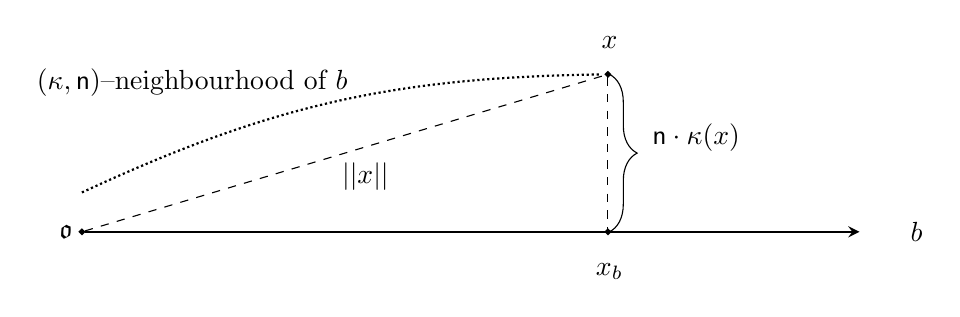
\begin{tikzpicture}
 \tikzstyle{vertex} =[circle,draw,fill=black,thick, inner sep=0pt,minimum size=.5 mm] 
[thick, 
    scale=1,
    vertex/.style={circle,draw,fill=black,thick,
                   inner sep=0pt,minimum size= .5 mm},
                  
      trans/.style={thick,->, shorten >=6pt,shorten <=6pt,>=stealth},
   ]

 \node[vertex] (a) at (0,0) {};
 \node at (-0.2,0) {$\go$};
 \node (b) at (10, 0) {};
 \node at (10.6, 0) {$b$};
 \node (c) at (6.7, 2) {};
 \node[vertex] (d) at (6.68,2) {};
 \node at (6.7, 2.4){$x$};
 \node[vertex] (e) at (6.68,0) {};
 \node at (6.7, -0.5){$x_{b}$};
 \draw [-,dashed](d)--(e);
 \draw [-,dashed](a)--(d);
 \draw [decorate,decoration={brace,amplitude=10pt},xshift=0pt,yshift=0pt]
  (6.7,2) -- (6.7,0)  node [black,midway,xshift=0pt,yshift=0pt] {};

 \node at (7.8, 1.2){$\nn \cdot \kappa(x)$};
 \node at (3.6, 0.7){$||x||$};
 \draw [thick, ->](a)--(b);
 \path[thick, densely dotted](0,0.5) edge [bend left=12] (c);
\node at (1.4, 1.9){$(\kappa, \nn)$--neighbourhood of $b$};
\end{tikzpicture}
\caption{A $\kappa$-neighbourhood of a geodesic ray $b$ with multiplicative constant $\nn$.}
\end{figure}
\end{definition}

\begin{definition} [$\kappa$-Morse I, $\kappa$-Morse II] \label{D:k-morse} \label{Def:Morse} 
Let $Z \subseteq X$ be a closed set, and let $\kappa$ be a concave sublinear function. 
We say that $Z$ is \emph{$\kappa$-Morse} if one of the following equivalent (see Proposition 3.10 \cite{QRT2})  condition holds:
\begin{enumerate}

\item[I.] (\emph{$\kappa$-strongly Morse}) There exists a proper function 
$\mm_Z : \mathbb{R}^2 \to \mathbb{R}$ such that for any sublinear function $\kappa'$ 
and for any $r > 0$, there exists $R$ such that for any $(\qq, \sQ)$-quasi-geodesic ray $\beta$
with $\mm_Z(\qq, \sQ)$ small compared to $r$, if 
$$d_X(\beta_R, Z) \leq \kappa'(R)
\qquad\text{then}\qquad
\beta|_r \subset \calN_\kappa \big(Z, \mm_Z(\qq, \sQ)\big)$$
%The function $m_Z$ will be called a $\emph{Morse gauge}$ of $Z$. 


\item[II.](\emph{$\kappa$-weakly Morse})  There is a function $\mm'_Z \from \RR_+^2 \to \RR_+$ so that if $\beta \from [s,t] \to X$ is a $(\qq, \sQ)$--quasi-geodesic with end points 
on $Z$ then
\[
[s,t]_{\beta}  \subset \calN_{\kappa} \big(Z,  \mm'_Z(\qq, \sQ)\big). 
\]
\end{enumerate}
\end{definition} 

\begin{remark}
By taking the maximum function of $\mm_Z, \mm'_Z,$ we may and will always assume that both conditions hold for the same $\mm_Z$, which we refer to as the $\kappa$-Morse gauge. Further,
\begin{equation} 
\mm_Z(\qq, \sQ) \geq \max(\qq, \sQ). 
\end{equation} 
\end{remark}

\begin{definition} \label{weakprojection}
Let $(X, d_X)$ be a proper geodesic metric space and $Z \subseteq X$ a closed subset, and let 
$\kappa$ be a concave sublinear function. A map $\pi_{Z} \from X \to \mathcal{P}(Z)$ is a $\kappa$-\emph{projection}  if there exist constants $D_{1}, D_{2}$, depending only on $Z$ and $\kappa$, such that for any points $x \in X$ and $z \in Z$, 
\[
\diam_X(\{z \} \cup \pi_{Z}(x)) \leq D_{1} \cdot d_X(x, z) + D_{2} \cdot \kappa(x).
\]
\end{definition}

A $\kappa$-projection differs from a nearest point projection by a uniform multiplicative error and a sublinear additive error. In particular, the nearest point projection is a $\kappa$-projection. Indeed, for $z \in Z$ and $w \in \pi_Z(x)$, we have
\[
d(z, w) \leq d(z, x) + d(x, w) \leq 2d(z, x).
\]
\begin{theorem}\label{A-sublinearlyequivalence}
Let $(X, \go)$ be a proper geodesic metric space with a fixed basepoint and let $\alpha$ be a quasi-geodesic
ray in $X$. Let $\pi$ be any $\kappa$-projection from $X$ to $\alpha$ in the sense of Definition~\ref{weakprojection}.
Then if $\alpha$ is $\kappa$-weakly Morse, then it is $\kappa'$-weakly contracting with respect to $\pi$ for some sublinear function $\kappa'$.
\end{theorem}


\begin{definition}[sublinear equivalence classes in $\pka X$] \label{Def:Fellow-Travel}
Let $\beta$ and $\gamma$ be two quasi-geodesic rays in $X$. If $\beta$ is in some 
$\kappa$--neighbourhood of $\gamma$ and $\gamma$ is in some 
$\kappa$--neighbourhood of $\beta$, we say that $\beta$ and $\gamma$ 
\emph{$\kappa$--fellow travel} each other. This defines an equivalence
relation on the set of quasi-geodesic rays in $X$ (to obtain transitivity, one needs to change $\nn$ of the associated $(\kappa, \nn)$--neighbourhood). 
\end{definition}

We denote the equivalence class 
that contains $\beta$ by $[\beta]$. We say two quasi-geodesic rays $\alpha, \beta$ \emph{sublinearly fellow-travel} if as $r \to \infty$, 
\[\lim_{r \to \infty} \frac{d(\alpha_r, \beta_r)}{r} = 0.\]

It is established in \cite{QRT2} that suppose $\alpha$ is a $\kappa$-Morse quasi-geodesic ray and suppose $\beta$ is a sublinearly Morse quasi-geodesic ray that sublinearly fellow travels $\alpha$ then $\beta$ $\kappa$-fellow travels $\alpha$. Thus it is a generalization of Gromov hyperbolicity in the sense that in these set of directions sublinear fellow traveling implies uniform sublinearly fellow travel. 

\begin{definition}[Sublinearly Morse boundary]
Let $\kappa$ be a sublinear function as specified in Section~\ref{subfunction} and let $X$ be a proper geodesic space.
\[\pka X : = \{ \text{ all } \kappa\text{-Morse quasi-geodesics } \} / \text{sublinear-fellow traveling}\]
%We define the topology of $\pka X$ in Section~\ref{coarsetop}.
\end{definition}



\subsubsection{A coarse cone topology on $\pka X$}\label{coarsetop}


 We equip $X$ with a topology which is 
a coarse version of the visual topology. In visual topology, if two geodesic rays fellow travel for a long time, then they are ``close''. In this coarse version, if two geodesic rays and all the quasi-geodesic rays in their respect equivalence classes remain close for a long time, then they are close. Now we define it formally. First, we say a quantity $\sD$ \emph{is small compared to a radius $\rr>0$} if 
\begin{equation} \label{Eq:Small} 
\sD \leq \frac{\rr}{2\kappa(\rr)}. 
\end{equation} 

\begin{definition}[Topology on $\pka X$]\label{openset}
Let $\bfa \in X$ and $\alpha_0 \in \bfa$ be 
the unique geodesic in the class $\bfa$. Define $\calU_{\kappa}(\bfa, \rr)$ to be the set of points $\bfb$ such that for any $(\qq, \sQ)$-quasi-geodesic of $\bfb$, denoted  $\beta$, 
such that $\mm_{\beta}(\qq, \sQ)$ is small compared to $\rr$, satisfies 
\[
\beta|_{\rr} \subset \calN_{\kappa}\big(\alpha_{0}, \mm_{\alpha_{0}}(\qq, \sQ)\big).\]

Let the topology of $\pka X$ be the topology induced by this neighbourhood system. The following fact shows that a $\kappa$-boundary is well defined with respect the associated group.
\end{definition}


\begin{figure}[H]
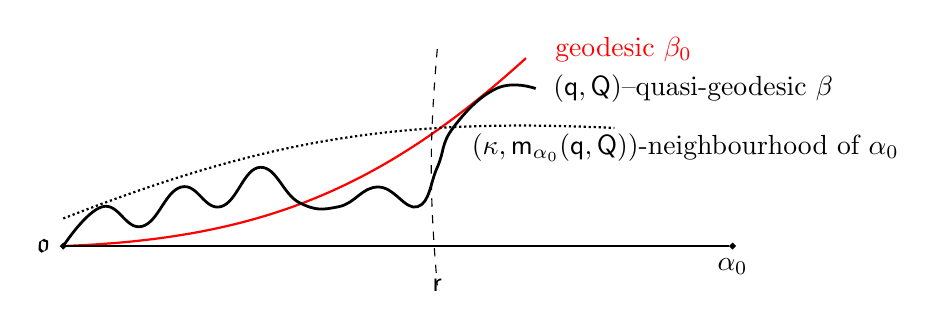
\begin{tikzpicture}[scale=0.5]
 \tikzstyle{vertex} =[circle,draw,fill=black,thick, inner sep=0pt,minimum size=.5 mm]
 
[thick, 
    scale=1,
    vertex/.style={circle,draw,fill=black,thick,
                   inner sep=0pt,minimum size= .5 mm},
                  
      trans/.style={thick,->, shorten >=6pt,shorten <=6pt,>=stealth},
   ]

  \node[vertex] (o) at (-10,0)  [label=left:$\go$] {}; 
  \node (o1) at (2, 5)[label=right:\color{red} geodesic $\beta_{0}$] {}; 
  \draw[thick, red]  (o) to [ bend right=20] (o1){};
  \node[vertex] (a) at (7,0)  [label=below:$\alpha_{0}$] {};
 \path[thick, densely dotted](-10,0.7) edge [bend left=12] (4, 3){};
 \node at (5.8, 2.5){$(\kappa, \mm_{\alpha_{0}}(\qq, \sQ))$-neighbourhood of $\alpha_{0}$};

       \node (a1) at (-1, 5) {}; 
   \node at (6,4) { $(\qq, \sQ)$--quasi-geodesic $\beta$};  
  \draw[dashed]  (-0.5, 5) to  [bend right=5] (-0.5, -1){};
  \node at (-0.5, -1){$\rr$};
 %   \draw[dashed](b)--(c){};$\rr$
   %     \draw[dashed](b)--(d){};

   \draw[thick]  (o)--(a){};
  
       
  \pgfsetlinewidth{1pt}
  \pgfsetplottension{.75}
  \pgfplothandlercurveto
  \pgfplotstreamstart
  \pgfplotstreampoint{\pgfpoint{-10cm}{0cm}}  
  \pgfplotstreampoint{\pgfpoint{-9cm}{1cm}}   
  \pgfplotstreampoint{\pgfpoint{-8cm}{0.5cm}}
  \pgfplotstreampoint{\pgfpoint{-7cm}{1.5cm}}
  \pgfplotstreampoint{\pgfpoint{-6cm}{1cm}}
  \pgfplotstreampoint{\pgfpoint{-5cm}{2cm}}
  \pgfplotstreampoint{\pgfpoint{-4cm}{1.1cm}}
  \pgfplotstreampoint{\pgfpoint{-3cm}{1cm}}
  \pgfplotstreampoint{\pgfpoint{-2cm}{1.5cm}}
  \pgfplotstreampoint{\pgfpoint{-1cm}{1cm}}
    \pgfplotstreampoint{\pgfpoint{-0.5cm}{2cm}}
      \pgfplotstreampoint{\pgfpoint{-0.1cm}{3cm}}
        \pgfplotstreampoint{\pgfpoint{1cm}{4cm}}
          \pgfplotstreampoint{\pgfpoint{2cm}{4cm}}
  %\pgfplotstreampoint{\pgfpoint{5cm}{7cm}}
  \pgfplotstreamend 
  \pgfusepath{stroke}
       
  \end{tikzpicture}
 
  \caption{ $\bfb \in \calU_{\kappa}(\bfa, \rr)$ because the quasi-geodesics of $\bfb$ such as $\beta, \beta_{0}$ stay inside the associated $(\kappa, \mm_{\alpha_{0}}(\qq, \sQ))$-neighborhood of $\alpha_{0}$ (as in Definition~\ref{Def:Neighborhood}), up to distance $\rr$. }
 \end{figure}













\begin{comment}
\begin{theorem} [\cite{QRT2}]
Let $X, Y$ be a proper metric space and let $\kappa$ be a sublinear function. The $\kappa$--boundaries of $X, Y$ are denoted $\pka X, \pka Y$. Any quasi-isometry from $X$ to $Y$ induces a homeomorphism between $\pka X$ and $\pka Y$.
\end{theorem}


%%%%%%%%%%%%%%%%%%%%%%%%%%%%%%%%%%%%%%%%%%%%%%%%%%old stuff



\end{comment}

\subsection{First passage percolation} \label{fpp}
 We consider a connected non-oriented graph $X$, whose set of vertices (resp. edges) is denoted by $V$ (resp. E). For every function $\omega: E \rightarrow(0, \infty)$, we equip $V$ with the weighted graph metric $d_{\omega}$, where each edge $e$ has weight $\omega(e)$. In other words, for every $v_{1}, v_{2} \in V, d_{\omega}\left(v_{1}, v_{2}\right)$ is defined as the infimum over all path $\gamma=\left(e_{1}, \ldots, e_{m}\right)$ joining $v_{1}$ to $v_{2}$ of $|\gamma|_{\omega}:=\sum_{i=1}^{m} \omega\left(e_{i}\right)$. Observe that the graph metric on $V$ corresponds to the case where $\omega$ is constant equal to 1 , we shall simply denote it by $d$. We consider a probability measure on the set of all weight functions $\omega$. We let $\nu$ be a probability measure supported on $[0, \infty)$. Our model consists in choosing independently at random the weights $\omega(e)$ according to $\nu$. More formally, we equip the space $\Omega=[0, \infty)^{E}$ with the product probability that we denote by $P$. In this project we always assume that $\nu({0})=0$, but generally we do not assume that the support of $\nu$ is bounded away from zero.

 Let $d(\gamma, \go)$ denote the distance between $o$ and the set of vertices $\{\gamma(0), \gamma(1), \ldots\}$. That is 
 \[d(\gamma, \go) : = \inf\bigg\{d(v, \go) : v \in \{\gamma(0), \gamma(1), \ldots\}  \bigg\} \]
%${ }^{2}$ Indeed, observe that Lemma 2.5 implies that X_{\omega}$ is a.e. locally finite in the sense that $d_{\omega}$-bounded subsets of vertices are finite.The hypothesis $E(\omega_{e})<\infty$ is used (only) in proving the follow facts \cite{BT17}.
The following two results (Proposition~\ref{BT1} and ~\ref{extension}) along with the lemma ~\ref{lemma2.13} established upper and lower bounds for how distance can be perturbed under first passage percolation. Proposition ~\ref{BT1} is established in \cite{BT17}. Proposition \ref{extension} is a generalization of  Lemma 2.5 in \cite{BT17}. 

\begin{proposition}\cite{BT17}\label{BT1}
Let $X$ be a connected graph, and let $\gamma$ be a self-avoiding path. Assume $0<b=\mathbb{E} \omega_{e}<\infty$. Then for a.e. $\omega$, there exists $r_{0}=r_{0}(\omega)$ such that for all $i \leq 0 \leq j$,

$$
\ell_{\omega}(\gamma([i, j]) \leq 2 b(j-i)+r_{0}
$$
\end{proposition} 
\begin{lemma}[Lemma 2.4 \cite{BT17}] \label{lemma2.13} Let $X$ be an infinite connected graph with bounded degree and assume that $\nu({0})=0.$ There exists an increasing function $\alpha:(0,\infty)\to (0,1]$ such that $\lim_{t\to0}\alpha(t) = 0,$ and such that for all finite path $\gamma$ and all $\epsilon>0,$
$$\mathbb{P}\big(\ell_\omega(\gamma)\leq \epsilon\cdot \ell(\gamma)\big) \leq \alpha(\epsilon)^{\ell(\gamma)}.$$
\end{lemma}

\begin{proposition}\label{extension}\label{BT2}
 Let $X$ be an infinite connected graph with bounded degree, and let $\go$ be some vertex of $X$. Assume $\nu(\{0\})=0$. Then for every constant $D$, there exists $c>0$ such that for a.e. $\omega$, there exists $r_{1}=r_{1}(\omega)$ such that for all finite path $\gamma$ such that $d(\gamma, o) \leq D \cdot \ell(\gamma)$, one has

\[ \ell_\omega(\gamma)\geq c(D) \cdot \ell(\gamma)-r_{1}\]
Furthermore, $c(\param)$ is an decreasing function.
\end{proposition}
\begin{proof}
Let $q$ be an upper bound on the degree of $X$, for simplicity, suppose $q\geq 2$ and let $n\geq 1$ be some integer. Suppose $\gamma$ is a path satisfying $d(o,\gamma) \leq D \cdot \ell(\gamma) = Dn$. Then the number of vertices in the ball $B(\go, Dn)$ is, 
\[|B(\go, Dn)| \leq 1+q \cdot \displaystyle\sum_{i=1}^{Dn-1}(q-1)^{i}\leq \displaystyle\sum_{i=0}^{Dn-1}(q+1)^i \leq (q+1)^{Dn+1}.\]Now possible number of paths of length $n$, starting in the ball $B(\go,Dn)$ is \[P_{n,D} \leq q\cdot (q-1)^{n-1}\cdot (q+1)^{Dn+1} \leq (q+1)^{(D+1)n+1} \]
Suppose $\alpha(t)$ be the increasing function with $\lim_{t\to 0} \alpha(t)=0$ in the Lemma ~\ref{lemma2.13}. Now define a function $\beta:(0,1] \to (0,\infty)$ such that,
\[\beta(t):= \sup \{x \in(0,\infty) : \alpha(x) \leq t \}.\] 
The function  is well defined since for every $t$ there exists $\delta_t>0$ such that $\alpha(x) \leq t$ wherever $x \in [0,\delta_t]$. Therefore, $[0,\delta_t] \subset \{x \in(0,\infty) : \alpha(x) \leq t \}$. Moreover, $\beta$ is non-decreasing and right continuous. Let, $C(D)$ be a function defined as $$C(D)=\beta(\frac{1}{q^{D+1}})$$
As a function of $D$, $C(D)$ is decreasing. Moreover by definition, $\alpha(C(D)\leq \frac{1}{q^{D+2}}$. Let us consider the following event, 
\[
A_{i,n,D}: = \{ \text{there exists some path $\gamma_i$ of length $n$, with $d(o,\gamma_i) \leq Dn$, and $\ell_\omega(\gamma_i)\leq c(D)\cdot \ell(\gamma_i)$\}}.\] 
By Lemma ~\ref{lemma2.13} $\mathbb{P}(A_{i,n,d}) \leq \alpha(C(D))^n\leq \frac{1}{q^{Dn+n}}$. There are up to $(q+1)^{(D+2)n}$ possible number of paths. Hence, the probability of at least one of these paths satisfies this property is, 
\begin{align*}
\mathbb{P}\left(\bigcup_{i=1}^{(q+1)^{(D+1)n+1}} A_{i,n, D}\right) &\leq \sum_{i=1}^{(q+1)^{(D+1)n+1}} \mathbb{P}m(A_{i,n, D})\\
&\leq (q+1)^{(D+1)n+1} \cdot \frac{1}{(q+1)^{Dn+2n}} \\
&= \frac{1}{(q+1)^{n-1}}.
\end{align*}
Thus $ \sum_{n=1}^\infty \frac{1}{(q+1)^{n-1}} < \infty$. Therefore, by the Borel-Cantelli lemma, the probability that this event happens infinitely often is 0.
\end{proof}
\begin{corollary}
Let $X$ be an infinite connected graph with bounded degree, and let $o$ be some vertex of $X$. Assume $\nu(\{0\})=0$. Let $\gamma:[0,n]\rightarrow X$ be any finite self avoiding path of length $n$, such that $ d(\gamma, o) \leq D \cdot n$. Then the image of $\gamma$ in $X_\omega$, is a quasi-isometric image of $\gamma$ whose constants depends only on $\omega$, i.e. there exists constants $q(\omega),Q(\omega)$ such that,
\[
 \frac{1}{q} \cdot \ell(\gamma)-Q(\omega)\leq \ell_{\omega}(\gamma) \leq q \cdot \ell(\gamma)+Q(\omega)
\]

\end{corollary}
\begin{proof}
Let $Q(\omega):= \max \{ r_{1}(\omega), r_{0}(\omega) \}$ and let $q: = \max \{2b,\frac{1}{c(D)}\}$ then by Propositions ~\ref{BT1}, ~\ref{BT2} we have the desired inequalities both sides.
\end{proof}


Now take the union of all $\kappa$-Morse boundaries and it is established in \cite{QRT2} that the topology on them are consistent with each other and in fact there exists a natural topology on the set of all sublinearly Morse directions, of which all $\kappa$-boundaries are subspaces with subspace topology.
\begin{definition}
Let $\partial_s X$ denote the set of all sublinearly Morse quasi-geodesic rays, up to sublinear fellow travelling. We refer to this as the \emph{Sublinearly Morse boundary}.
\end{definition}
\begin{definition}
The topology on $\partial_s X$ is defined as follows: let $\beta$ be a $\kappa$ Morse sublinearly quasi-geodesic ray for some $\kappa$. An equivalence class $\bfa \in 
\ps X$ belongs to $U(\beta,r)$ if, for any $(q,Q)$-quasi-geodesic ray $\alpha \in \bfa$,
where $m_\beta(q,Q)$ is small compared to $r$ with respect to $\kappa$, we have the inclusion
\[ \alpha|r \ \subset N_\kappa( \beta,m_\beta(q,Q)).\]
\end{definition}
An open neighborhood $\calV$ of a point $\bfb \in \ps X$ contains all $\kappa'$-Morse quasi-geodesic rays that in the ball of radius $r$ around quasi-geodesic rays of $\bfb$, behaves as if they are a member of $\bfb$. It is established in \cite{QRT2} that with this topology the space $\ps X$ is metrizable and contains each $\pka X$ as a topological subspace.
% Let $X$ be an infinite connected graph with bounded degree and assume that $\nu(\{0\})=0$. There exists an increasing function $\alpha:(0, \infty) \rightarrow(0,1]$ such that $\lim _{t \rightarrow 0} \alpha(t)=0$, and such that for all finite path $\gamma$ and all $\varepsilon>0$,
%\[
%P\left(|\gamma|_{\omega} \leq \varepsilon|\gamma|\right) \leq \alpha(\varepsilon)^{|\gamma|}
%\]

%\begin{corollary}
%There exists a constant $D'$ such that if 
%\[d_\omega(\gamma_\omega, \go_\omega) < D \ell_\omega(\gamma),\]
%Then there exists a c depending on $D'$ such that 
%\[ P\left(|\gamma|\geq \varepsilon|\gamma_\omega|\right) \leq %\alpha(\varepsilon)^{|\gamma|}\]
%\end{corollary}
%\begin{proof}
%\textcolor{red}{insert the proof}
%\end{proof}

    











\section{middle-recurrence of sublinear lines}
In this section we study the middle-recurrence property of sublinearly Morse bi-infinite lines and use it to characterize sublinearly Morse directions and bi-infinite lines. Let $\gamma$ be a sublinearly Morse set. The middle recurrent property concerns the location of paths with endpoints on $\gamma$ as opposed to the location of quasi-geodesic segments with endpoints on $\gamma$. 

By a \textit{path} we mean the continuous image of an interval $[a, b]$ in $X$. In this paper, we assume all paths to be an embedding of an interval and thus are  self-avoiding. This assumption makes the argument shorter.
Given a path $\alpha$ with endpoints $x, y$, suppose $\ell(\alpha)$ be the arc-length of $\gamma$ then  the \textit{slope} of $\alpha$ is defined to be 
\[ sl(\alpha):= \frac{\ell(\alpha)}{d(x,y)}  \]
where the arc-length of a continuous curve $\alpha: I \rightarrow X$ is defined as the infimum of the sum of the distances $d(\alpha(t_{i-1}), \alpha(t_i))$ over any partition $\{t_i\}_{i\geq0}$ of $I$.
\begin{definition}
Let $\gamma$ be set. We say that a $\gamma$ has the \textit{middle-recurrence property}  if for every $C\geq1$ there is a constant $c$ (depends on $C$ and $\beta$) such that the following holds: 
    for any path $P$ with endpoints $a,b \in \gamma$ satisfying $\ell(P)\leq Cd(a,b)$, intersects the $c\cdot \kappa$-neighborhood of the middle third of $\gamma[a,b]$ for some sublinear function $\kappa$. That is,
\[ P \cap \calN_{\kappa} (\gamma_{\frac 13[a,b]}, c )\neq \emptyset.\]
%Where, $\beta_{\frac{1}{3}[a,b]} := \biggl\{x\in \beta : \min \{d(x,a),d(x,b)\} \ge \frac{1}{3}\cdot d(a,b)\biggr\}$.


\end{definition}
Middle recurrence is first studied by \cite{DMS} and then corrected and further expanded by \cite{ADT}. Here we use an distance estimation lemma \cite[Lemma 3.3]{ADT} that gives an upper bound  of the distance between the end points of a path with fixed slope and other properties. Let $p$ be a path with end points $s$ and $e$. 

\begin{lemma}
Let $\beta$ be a $\kappa'$–radius-contracting quasigeodesic and suppose that $p$ is a path with the following properties:
\begin{itemize}
\item slope of $p$ is $D$
\item $p$ is at distance at least $K$  from $\beta$
\item The end points of $p$ are at distance exactly $K$ from $\beta$. 
\end{itemize}
Let $|p|: d= d(s, e)$ denote the distance between the endpoints of $p$. Then
\[ \frac{\kappa(K)}{2K} \geq \frac{1-(2K+\kappa'(K))/|p|}{D}\]
\end{lemma}

\subsection*{Notation}In the rest of this paper, if $\gamma$ is a geodesic line, then the restriction of $\gamma$ between two points $a, b\in \gamma$ is notated as $\gamma{[a, b]}$. Furthermore, if we are referring to a segment of this geodesic segment that starts at one third from the endpoint $a$ and ends at $\frac 23$ from the endpoint $a$ then we notate it as $\gamma_{\frac13 [a,b]}$. In general, if a geodesic segment $\alpha$ lies on a geodesic ray that emanates from the origin, then it is assumed that $\alpha_{[p, q]}$, where $0\leq p, q \leq 1$, lies between the fractions $p$ and $q$ starting from the point closer to the origin.

In \cite{JanaQing1}(Theorem A]) we have proved the following one sided Proposition:
\begin{proposition}[$\kappa$-Morse implies middle recurrence] \label{prop3.3}
Let $\gamma$ be a bi-infinite geodesic line. Assume that  $\gamma$ is $\kappa$-Morse with Morse gauge $M$. Let $P$ be any simple path with endpoints $a, b \in \gamma$ and such that $\ell(P) < C d(a, b)$. Then there exists a sublinear neighborhood of $\gamma$ depending only on $\gamma$ and $C$ such that 
\[ P \cap \calN_{\kappa'} (\gamma_{\frac13 [a,b]}, c(C, \beta)) \neq \emptyset.\]
Here $\kappa'$ is the contracting sublinear function of $\beta$.
\end{proposition}
% \begin{proof}
%     To proceed, let 
%     $\kappa'$ denote the contracting function of $\beta$ \cite{theorem ??}. By way of contradiction, suppose there does not exist any sublinear neighborhood of $\beta$ in which $p$ intersects the middle third. 
%   Then there exists a constant $c_1$ such that there exists a family of paths $\{p_i \}$ such that for arbitrarily large $t$, there exists a $p_i$ where $p_i(t)$ is outside of the $c_1$-linear neighborhood of the middle third of $p_i$. That is, 
%   Let 
%   \begin{equation}\label{linearnbd} 
%   LN(\beta, c_1) : = \{ x \in X | \, d(x, \beta) \geq c_1 \cdot d(\go, x)\}.
%   \end{equation}
%   Given any such $p_i$, let $p_i'$ be a connected segment of $p_i$ that connects points where $p_i$ exits the $c_1$-linear neighborhood of $\beta$ and does not intersect the middle third. By construction, with respect to points on $p_i'$, $\beta$ is at least $\kappa$-radius-contracting.
  
%   Secondly, suppose the end points of $p_i'$ are $(s'_i, e'_i)$, then
%   \[ d(s'_i, e'_i) \geq \frac 13 d(s_i, e_i)\]
%   Thus 
%   \[ \sl(p_i)' \leq 3 s\sl(p_i) \leq C.\]
%   Furthermore, we claim that for large enough $i$, 
%   $d(s_i, e_i)$ does not grow sublinearly with respect to 
%   $d(\go, s_i)$, otherwise, since slope of $p_i$ are bounded, eventually $p_i$ will not be outside of the linear neighborhood of of $\gamma$, thus there exists a constant $c_2>0$ where
%   \[
%    d(s_i, e_i) \geq c_2 d(\go, s_i).
%   \]
%   Therefore, a slight adaptation of the Lemma?? we get 
%   \[ \frac{\kappa(t)}{t} \geq \frac{1-(c_2' t +\kappa(t))/d(s'_i, e'_i)}{3C}\]
%   However, as $i \to \infty$, if $d(s'_i, e'_i)$ grows at most sublinearly with respect to $d(s_i, e_i)$, then eventually there will mid-third recurrence. Thus by construction, there exists $c_2$ such that for all $i$ large enough, $d(s'_i, e'_i) \geq c_3 t$ and thus there exists a uniform constant $D>0$ depending only on $C, c_1, c_2, c_3 \kappa \kappa'$ where 
%   \[
%   \frac{1-(c_3 t +\kappa(t))/d(s'_i, e'_i)}{3C} \geq D.
%   \]
%   Thus there exist a maximal $t$ for which the inequality holds, which is a contradiction as desired. 

% \end{proof}


% %Assume that $d(a, \go) < d(b, \go)$, the \emph{projective norm} of a finite path $P$ is defined as 
% %\[
% %\Norm{P}_\go: = \frac{d(a, b) }{d(b, \go)}.
% %\]
Now in the following proposition we will establish the other direction:
\begin{proposition}[Middle recurrence implies sublinearly Morse] \label{prop3.4}
 Let $\gamma$ be a geodesic ray. Suppose  there exist function $M \from \mathbb{R_{+}}\to\mathbb{R_{+}}$ and a sublinear function $\kappa$ such that the following holds:  
 \begin{itemize}
     \item for every self-avoiding path $P$ with slope $sl(P)<C$ and endpoints $a,b\in\gamma$,
\[
P \cap \mathcal{N}_\kappa \left(\gamma_{\frac13 [a,b]},\, M(C)\right)\neq \emptyset.
\]
 \end{itemize}
 Then $\gamma$ is sublinearly Morse. 
%  Let $\gamma$ be a geodesic ray, and let $P$ be a self avoiding path with endpoints $a, b$ on $\gamma$ with the following properties: 
% \begin{itemize}
% \item the slope of $P$: $sl(P) < C$
% %\item the projective norm :
% %\[ \Norm{P}_\go \geq c_2.\]
% \item There exists a family of constants $M \from \RR^2 \to \RR^2$ and a sublinearly function $\kappa$ such that \[ P \cap \calN_\kappa(\gamma_{\frac{1}{3}[a,b]}, M(c_1,c_2)) \neq \emptyset\] for some $c_1,c_2 \in \mathbb{R}.$

% \end{itemize}

\end{proposition}
Before giving the main proof of the proposition, we establish the following lemma. 
\begin{lemma}\label{middle rec quasi geodesic} (See figure ~\ref{middle rec lemma})
Let $\gamma$ be a geodesic and assume the hypotheses of Proposition \ref{prop3.4}. Let $p:I\to X$ be a continuous $(q,q)$--quasi-geodesic with endpoints $a,b\in\gamma$.
Fix
\[
d:=\max\left\{M\left(\frac{13q+2}{10},0\right),\,1\right\}.
\]
If $\pp'\subset P$ is a sub path that remains at most distance $d\cdot\kappa(t)$ from $\gamma$ and its endpoints
$a'$ and $b'$ satisfy,
$
d(a',b') \geq 12d \cdot \max \{ \kappa(\Norm{a'},  \kappa(\Norm{b'} \}
$
then
\[
\pp'\cap \mathcal N_{\kappa}(\gamma,d)\neq\emptyset.
\]
\end{lemma} 
\begin{remark}
  Although we stated the lemma for a $\pp$ being a $(q,q)$-quasi-geodesic, the conclusion holds for an arbitrary quasi-geodesic: by the taming lemma (\cite{BH1}, Lemma III.H.1.11]), any quasi-geodesic can be replaced by a tame one (with controlled constants).  
\end{remark}
\begin{figure}[H] 

\includegraphics[height=5cm,width=13cm]{middle_rec_lemma.png} 
\caption{ if $a',b'$ are $\kappa-$separated then a sub path $\pp'$ intersects a $\kappa'$ neighborhood of $\gamma.$ \label{middle rec lemma}} 
\end{figure} \begin{proof}
Suppose, $A=A(a',b')=  \max \{\kappa(||a'||), \kappa (||b'||)\}$. Let \( x, y \in \gamma \) such that \( d(x, a') \leq d \cdot \kappa(||a'||) \), \( d(y, b') \leq d \cdot \kappa(||b'||)\). Let \( \omega \) be the concatenation \( [x, a'] \cdot \pp' \cdot [b', y] \). From the given hypothesis, we have the following estimates:
\begin{equation}
   d(x, y)\geq d(a',b') - d(a',x) -d(b'y) \geq 12d \cdot A(a',b')-d \kappa(||a'||)-d \kappa(||b'||)  \label{eq2}
\end{equation}
Therefore we have,
\begin{equation}
 d(x, y)\geq 10 d \cdot A(a',b') \label{eq3}
\end{equation} On other hand, since $d(a',b)\geq 12d \cdot A(a',b')$ we get,
\begin{equation}
d(a',b') - 2d \cdot A(a',b') \ge \frac{5}{6}\,d(a',b') .
\label{eq4}
\end{equation}
 Since $\pp$ is $(q,q)$ quasi-geodesic we can assume that $\Norm{\pp'} \leq q \cdot d(a',b') +q$.
Now we compute the slope of $\omega$:
\begin{align*}
\frac{\ell(\omega)}{d(x, y)} &\leq \frac{\Norm{\pp'}+ d(a',x)+d(b',y)}{d(x,y)}\\
&\leq\frac{\Norm{\pp'}+ d\cdot \kappa(\Norm{a'})+ d \cdot \kappa(\Norm{b'})}{d(x,y)}\\
&\leq \frac{\Norm{\pp'}}{d(a',b')-d \cdot \kappa(\Norm{a'})-d \cdot \kappa(\Norm{b'})}+ \frac{d\cdot \kappa(\Norm{a'})+ d \cdot \kappa(\Norm{b'})}{d(x,y)} \\
&\leq \frac{q \cdot d(a',b')+q}{d(a',b')-2d \cdot A(a',b')}+ \frac{2d \cdot A(a',b')}{10d \cdot A(a',b')} \qquad\text{(by equation~\ref{eq3})}\\ 
&\leq \frac{q \cdot d(a',b')+q}{\frac{5}{6}d(a',b')}+ \frac{1}{5}  \qquad\text{(by equation~\ref{eq4})}\\
&\leq \frac{13q+2}{10}
\end{align*}
Thus, $\omega$ has bounded slope. Hence, by middle recurrence, there is a point $c \in \pp'$ that intersects the $\kappa$-neighborhood of the middle third of $\gamma_{[x, y]}$ i.e. there exist $z \in \gamma_{\frac{1}{3}[x, y]}$ such that $d(c,z) \leq d \cdot \kappa(\Norm z).$
\newline \underline{\emph{Claim:} } $c$ belongs to $\pp'.$
\newline \underline{\emph{proof of the claim:}} Suppose without loss of generality $c$ is on the geodesic joining $a'$ and $x$. By definition ~\ref{def:middle recurrent} and equation ~\ref{eq3} we have, 
\begin{equation}
    3d(z,x) \geq  d(x,y) \geq 10d \cdot A(a',b'). \label{eq5}
\end{equation}
Note that, $\Norm c \leq \Norm {a'}+ d(a',x) \leq 2 \Norm {a'}.$ Hence, by triangle inequality we have, 
\begin{align*}
  3d(z,x) &\leq d(z,c)+d(c,x)\\
  & \leq d \cdot \kappa(\Norm c)+d \cdot \kappa(\Norm a')\\
  & \leq 9d\cdot A(a',b')
\end{align*}
which is a contradiction to equation ~\ref{eq5}. Hence, the lemma follows.


\end{proof}
\subsection*{Proof of Proposition ~\ref{prop3.4}}

Let, $Q =\{t\in I:d(\pp(t), \gamma) \leq d \cdot \kappa(\Norm{\pp(t)})\}$. $Q^c$ is a collection of disjoint unions of open intervals in $\mathbb{R}$. If $(t,t') \in Q^c$ then \[d (\pp(t),\pp(t')) < 12d \cdot A(\pp(t),\pp(t')).\] If $\eta \in Q^c$ then $\eta \in (t,t')\subset Q^c$ for some $t,t' \in \mathbb{R}$. We have then,
 \[d(\pp(\eta), \pp(t))< d \cdot  \max \{ \kappa(\Norm {\pp(\eta)}, \kappa(\Norm{\pp(t))}.\} \]
 Otherwise it contradicts Lemma ~\ref{middle rec quasi geodesic}.
 Therefore, \[d(\pp(\eta),\gamma) < d(\pp(\eta), \pp(t))+ d \cdot \kappa(\Norm{\pp(t))} < 12d \cdot  A(\pp(\eta), \pp(t))+d \cdot \kappa(\Norm{\pp(t)}).\]
 Since $ d(\pp(\eta), \pp(t)) \leq 12d \cdot \max \{ \kappa(\Norm {\pp(\eta)}, \kappa(\Norm{\pp(t))}\}$ then by Lemma ~\ref{lemma2.3} 
 there exist $D >0$ such that, 
 $$\kappa(\Norm {\pp(t))} \le D \cdot \kappa(\Norm{\pp(\eta))}$$ 
Therefore, \[d(\pp(\eta),\gamma) \leq 12d\cdot (\kappa(\Norm {\pp(\eta)})+D\cdot \kappa(\Norm \pp(\eta))+ d \cdot D\cdot \kappa(\Norm {\pp(\eta)}).\]
This implies, \[d(\pp(\eta),\gamma) \leq d \cdot (13 D+12) \cdot  \kappa(\Norm {\pp(\eta)}).\]
Thus, there exists a sublinear function $\kappa'$ depends on $\kappa$ such that $\pp \subset \calN_{\kappa'}(d, \gamma)$. Hence, Proposition ~\ref{prop3.4} follows.
%\textcolor{red}{Not needed: }
%The claim implies that the complement of \( Q \) in \( \text{dom}(q) \) is a collection of open intervals, each of whose image in \( X \) has length at most \( 4\kappa_1
%\cdot d/t + \kappa_1 \). Hence,
%\( q(N) \leq d + 4\kappa_1 d/t + \kappa_1 (\gamma) \), as required.
%Given the claim, the conclusion because the whole line is only skipped by $12d$ and thus can be at most 12 times $\kappa$-neighbhorood. The middle 3rd implies the claim because make 12 big enough to make the splicing a good path with good slope. Thus we have shown that all paths of slope bounded above by $c_1$ is contained in a sublinearly neighborhood of $\gamma$. Since any $(q, Q)$-quasi-geodesic segments with endpoints on $\gamma$ are paths of bounded slope, the statement follows.
\hfill $\blacksquare$\\
Now we can conclude the following theorem, as Proposition ~\ref{prop3.3}, Proposition ~\ref{prop3.4} establish the statement in each direction.
\begin{theorem}
Let $X$ be a proper geodesic metric space. Let $\beta$ be a $\qq$-quasi-geodesic ray. Then $\beta$ is sublinearly Morse if and only if $\beta$ is $\kappa$-middle recurrent for some $\kappa$.
\end{theorem}


% \begin{corollary}\label{box}
% Let $\gamma$ be a sublinearly Morse geodesic ray. Then there exists a sublinear function $\kappa^{\rm path}$ and a function $p: \R^2 \to \R$ such that for any $c, L>0$. Suppose $\pp$ be a path with local slope bound $L$ (i.e. for any subpath $\pp'$ of $\pp$, $sl(\pp')\leq L$) and starting distance $\leq cL$ is contained in a $p(c,L)\kp(t)$-neighborhood of $\gamma$. 
% \end{corollary}


% However, since there exists a sublinear function $\kappa'$ such that every point of $\gamma_0$ is in a  $\kappa'$-neighborhood of
% $\gamma_\omega$, for each $c_i$,  there exists a point $d_i \in \gamma_0$ and a pair of points $a_i, b_i \ in \gamma_omega$ such that 
% \[d(d_i, a_i)\leq \kappa'(d_i), d(d_i, a_i)
% \leq \kappa'(d_i).\]
% Thus 
% \[d(a_i, b_i)< 2\kappa'(d_i)\]
% and the path lengths
% \begin{equation}\label{pathlength}
% d_{\gamma_\omega}(a_i, b_i) \geq c' d(\go, d_i)
% \end{equation}
% Now consider the distance between $a_i, b_i$ in $X$. In $X$, $d_i$ is also sublienarly close to $a_i, b_i$, which implies by triangle inequality that 
% \[d_X(a_i, b_i) < \kappa(d_i)\]
% and this distance is in fact the path length since $\gamma$ is a geodesic. This contradicts equation ~\ref{pathlength}. Therefore, no such sequences of $c_i$ and $c$ exist.


% Let $\gamma$ be a sublinearly Morse geodesic ray.

% \begin{enumerate}
% \item If a path $P$ with endpoints $x, y$ is of slope $L$ and starting distance $\leq cL$ is contained in a $p(c,L)\kp(t)$-neighborhood of $\gamma$, then $[x,y ]_\gamma$, the geodesic segment is is contained in a $D(c, L, \kappa)$-neighborhood of $P$ where
% \[ D(c, L, \kappa): = 2p(c,L)\kp(t)+2.\]
% \item Furthermore, in $X_\omega$, we have that $\gamma_\omega$ and the geodesic ray $\gamma_0$ are in sublinear neighborhoods of each other.
% \end{enumerate}
% \begin{proof}
% We first prove part (1). Consider a sequence of points on $P$ that are distance at most apart and including the endpoints $x, y$. Denote these points $a_1, a_2,...a_n$ and their projections on $[x,y ]_\gamma$ as $a^{\gamma}_1, a^{\gamma}_2,...a^{\gamma}_n$. Let $x \in [x,y ]_\gamma$ be any point on $[x,y ]_\gamma$. Then there exists $a_i$ and $a_{i+1}$ such that $x$ lies on a geodesic segment with endpoints 
% $a^{\gamma}_i$ and $a^{\gamma}_{i+1}$. Since 
% \[ d(a_i, a^{\gamma}_i) < \kappa(|a_i|)\]
% we have 
% \[ d(a^{\gamma}_i, a^{\gamma}_{i+1})\leq \kappa(|a_i|)+1 +\kappa(|a_{i+1}|)\]
% Thus any point on the geodesic segment $[a^{\gamma}_i, a^{\gamma}_{i+1}]$ is within distance $2\big(\kappa(|a_i|)+1 +\kappa(|a_{i+1}|)\big)$ from some point on $P$. Since this is true for every point on $[x, y]$, we have that $[x, y]$ is in a sublinear neighborhood of $P$.

% For (2), by way of contradiction, suppose $\gamma_\omega$ and $\gamma_0$ travels linearly far away from each other. Then the segments realizing the sublinearly growing distances in $X$ are mapped to linearly growing segments in $X_\omega$, which is not possible by Proposition 2.12.
% \end{proof}
\section{Sublinearly Morse directions under first passage percolations}
Now we are equipped with the path charaterization of sublinearly Morse directions, we are ready to establish Theorem~\ref{introthm1} in this final section. Recall from Section~\ref{fpp} all relevant background of first passage percolation. In particular recall that we always assume $\nu({0})=0$. The first lemma shows that sublinear neighborhoods are preserved.
\begin{lemma}\label{neighborhood}
Let $X$ be a graph of bounded degree with a fixed base point. Let $\gamma$ be any geodesic ray in $X$ emanating from the base point. Then the set of $\omega$ that maps any sublinear neighborhood of any $\gamma$ in $X$ to a linear neighborhood in $X_\omega$ of $\gamma_\omega$ is a set of measure zero.
\end{lemma}
\begin{proof}
Suppose $\calN_\kappa(\gamma,n)$ be a sublinear neighborhood of $\gamma$ in $X$ for some sublinear function $\kappa$ and gauge $n$. Let $x \in \calN_\kappa(\gamma,n)$. Then by Proposition ~\ref{BT1}, \[d_\omega(x, \gamma) \leq b \cdot n \cdot \kappa(||x||) + r_o(\omega).\]
Consider $[\go,x]_\omega$ be the $\omega$-geodesic in $X_\omega$. Then the preimage of  $[\go,x]_\omega$ in $X$ satisfies the assumption of Proposition ~\ref{BT2}. Therefore, we get \[||x||_\omega=\ell_\omega([\go,x]_\omega) \geq c \cdot ||x||-r_1(\omega).\]
Hence for a.e. $\omega$ we have, 
\begin{align*}
d_\omega(x,\gamma) \leq  & \frac{b\cdot n}{c} \cdot \kappa(||x||_\omega+r_1(\omega))+r_0(\omega)\\
& \leq \bigg(\frac{b\cdot n}{c}+r_0(\omega)\bigg) \cdot \kappa'(||x||), \text{ where, $\kappa'(t)= \kappa(t+r_1(\omega))$.}
\end{align*}
Therefore, almost surely, FPP sends a sublinear neighborhood of a geodesic ray in $X$ to a sublinear neighborhood of the image ray in $ X_\omega$.  


% This follows from Proposition~\ref{BT1} and Proposition~\ref{BT2}, as every point $x$ in a sublinear neighborhood can be thought of as an endpoint of a geodesic segment $[\go x]$ where  $[\go x]$ satisfies the assumption of Proposition~\ref{BT2}. Thus the norm of every point in the sublinear neighborhood is sent to a point with additive and multiplicative error bounded above and below, which does not affect the sublinearity of the neighborhood.

\end{proof}
% Lemma~\ref{{neighborhood}} not only is important to establish a well-defined map (see Definition~\ref{maponray}) between sublinearly Morse boundaries of $X$ and $X_{\omega}$, but also allow us to make the following independent observation, which can be compared to \cite[Theorem 6.6]{MB1}. For the definition of visual boundary of a graph see Section~\ref{??}.
% \begin{proposition}
%     Let $X$ be an infinite graph with uniformly bounded degree. Then For $\go$ in $X$, for a.e. $\omega$, all $\omega$-geodesic rays (preimages of geodesic rays in $X_\omega$) starting at $\go$ converges to a unique point in the visual boundary of $X$. 
% \end{proposition}
% \begin{proof}
% \textcolor{red}{need to discuss}
%     Suppose $\alpha_\omega$ is a geodesic ray in $X_\omega$ starting at $\go$ and $\alpha$ be the preimage of $\alpha_\omega$ in $X$. For the way of contrary suppose the $\omega-geodesic$, $\alpha$ has two different accumulation points namely $\xi$, $\eta$ in visual boundary of $X$.
% \end{proof}
\begin{theorem} \label{37}
The image of a $\kappa$-Morse geodesic is almost surely sublinearly Morse. Specifically, let $\gamma$ be a $\kappa$-Morse geodesic ray emanating from a fixed base point $\go$ in $X$. Then for a.e. $\omega$ there exists $\kappa'$, depending on $\kappa$ and $\omega$ such that $\gamma_\omega$ is $\kappa'$-Morse.
\end{theorem}
\begin{proof}
Assume $\gamma^{\omega}\subset (X,d_{\omega})$ is not sublinearly Morse. Then there exist $(q,Q)$, a constant $c_{1}>0$, and a family of $(q,Q)$--quasi--geodesic segments 
$\{\alpha_i\}_{i\in\mathbb N}$ with endpoints $(s_i,e_i)$ on $\gamma^{\omega}$ such that for each $i$ there exists a point 
$x_i\in \alpha_i$ satisfying
\[
d_{\omega}(o,x_i)\ge i
\qquad\text{and}\qquad
d_{\omega}(x_i,\gamma^{\omega})\ge c_{1}\, d_{\omega}(o,x_i).
\]
In particular, $\alpha_i$ is not contained in the $c_{1}$--linear neighborhood of $\gamma^{\omega}$.

% Let $\gamma \in X$ be a $\kappa$-Morse geodesic ray. Consider $\gamma_\omega \subset X_\omega$. Suppose that 
% $\gamma_\omega$ is not sublinearly Morse, then there exists $(q, Q)$, $c_1 > 0$ and a family of $(q, Q)$-quasi-geodesic segments $\{\alpha_i \}$ with endpoints on $\gamma_\omega$ such that for each $i \in \NN$, there exists $\alpha_i$ whose starting point is of norm greater than $i$ and $\alpha_i$ is not contained in the $c_1$-linear neighborhood of $\gamma_\omega$.

% Because $\alpha_i$ is not contained in the neighborhood, they have to be linearly long compared to their distance to the origin, thus there exists a constant $c_2(c_1, q, Q)$ such that for all $\alpha_i$
% \[
% i<d(\alpha_i, \go) \leq c_2 |\alpha_i|.
% \]
Now consider the pre images of $\alpha_i$ (say, $\alpha_i^X)$ in $X$. For all $i$, the endpoints of $\alpha_i^X$ on $\gamma$ are $s_i,e_i$ respectively. We make the following claim:
\begin{claim}
Up to an infinite subsequence $\{i_k\}$, the base of $\alpha^X_{i_k}$ are bounded below by $c_3 \cdot d(\go, s_{i_k})$ for some $c_3$, i.e. there exists $c_3$ such that $d(s_{i_k},e_{i_k}) \geq c_3 \cdot d(s_{i_k}, \go). $ 
\end{claim}
\begin{proof} From the assumption we have $x_i \in  \alpha_i$ such that, \[d_\omega(x_i,\gamma_\omega) \ge c_1 \cdot d_\omega(\go,x_i).\]
On the other hand,  $d_\omega(\go,s_i) \le d_\omega(\go,x_i) + d_\omega(x_i,s_i) \le \big(\frac{1+c_1}{c_1}\big)\ d_\omega(x_i,s_i).$
 \text{Therefore,}
\begin{equation} \label{eq:upperbound}
   \ell_\omega(\alpha_i) \ge \frac{c_1}{1+c_1} \cdot d_\omega(\go,s_i).
\end{equation}

By Proposition ~\ref{BT2}, for a.e. $\omega$ we get,
\begin{equation} \label{eq:lowerbound}
    d_\omega(\go,s_i)\ge c \cdot d(\go,s_i)-r_1(\omega).
\end{equation}
    
Since, $\alpha_i$ is a $(q,Q)$ quasi-geodesic, we have,
\begin{equation} \label{eq:lengthbound}
 q \cdot d_\omega(s_i,e_i)+Q \ge \ell_\omega(\alpha_i).   
\end{equation}
Now, by combing Equations ~\ref{eq:upperbound}, ~\ref{eq:lowerbound}, ~\ref{eq:lengthbound} and using Proposition ~\ref{BT1}, there exists two constants $L_1,L_2$ (which depends on $\omega$) such that, \[d(s_i,e_i) \ge L_1 \cdot d(\go,s_i)-L_2.\]
By assumption, $d(s_i,\go) \rightarrow \infty$ as $i \rightarrow\infty.$ Therefore, for large $i$, we have \[d(s_i,e_i) \ge c_3\cdot d(\go,s_i).\]
    

% Because the pre image of end points of $\alpha_i$ are all endpoints of geodesic segments emanating at the basepoint, thus the distances $d(\go_\omega, s^i)$ and $d(\go_\omega, e_i)$ have linear upper and lower bounds. Thus the inverse map from $X_\omega$ to $X$ also has upper and lower bound for the distances $d(\go_\omega, s^i)$ and $d(\go_\omega, e_i)$. Therefore, for all large enough $i$, the base of $\alpha_i$ are mapped to a geodesic segment whose length is bounded below and above linearly with respect to $d(\go, s_i)$ thus also bounded below and above linearly with respect to $d(\go, s^X_i)$.
\end{proof}


\begin{claim} \label{39}
The paths $\alpha^X_i$ have bounded slope.
\end{claim}
\begin{proof}
Suppose otherwise, that as $i \to \infty$, the slope of $\alpha^X_i$ tends to infinity i.e. $\frac{\ell(\alpha_i^X)}{d(s_i,e_i)} \rightarrow \infty$. Therefore, there exists $R> 0$ such that $\ell(\alpha_i^X) \ge \frac{1}{c_3}\cdot d(s_i,e_i)$   Since the base grows linearly with respect to $d(\go, s^X_i)$, the lengths of the curves grows superlinearly with respect to the base and distance to the origin. Thus all but finite of $\{ \alpha^X_i \} $ satisfies the condition:
\[ d_X(\go, s^X_i) \leq \ell(\alpha^X_i).\]
By Proposition ~\ref{BT2}, for a.e. $\omega$ we have,
\begin{equation} \label{eq6}
 \ell_\omega(\alpha_i) \ge c \cdot \ell(\alpha_i^X) -r_1
\end{equation}
Hence by Equation ~\ref{eq6} and Proposition ~\ref{BT1}, \[sl(\alpha_i) = \frac{\ell_\omega(\alpha_i)}{d_\omega(s_i,e_i)} \geq \frac{ c \cdot \ell(\alpha_i^X) -r_1}{b \cdot d(s_i,e_i)+r_0} \]
Thus, $sl(\alpha_i)$ grows unboundedly as $i$ goes to infinity because the slope of the curves $\alpha_i^X$ goes to infinity in $X$. This is impossible as $\alpha_i$'s are quasi-geodesics in $X_\omega$. Therefore, it follows that the paths $\{\alpha^X_i\}$ also have bounded slopes.
\end{proof}
Thus the preimages all have bounded slope and by the path characterization, 
they all intersect the middle third of a sublinearly neighborhood. Which contradicts lemma~\ref{neighborhood}. Thus $\gamma_\omega$ is a sublinearly Morse set.
\end{proof}
\begin{remark}
The argument of Claim~\ref{39} makes it clear that we can only establish our main claim for sublinearly Morse boundary as opposed to for a specific $\kappa$-Morse boundary. 
\end{remark}
\subsection{Construction of the bijective map between sublinearly Morse boundaries} \label{Remark1}

First we observe that  a sublinear Morse geodesic ray can be mapped to a sublinearly Morse geodesic ray.
We first observe that one can always find a geodesic ray in a sublinear bound of the  set $\gamma_\omega$. This follows from Theorem 3.8 in \cite{JanaQing1}. 
Furthermore, the construction of the geodesic line is the following: consider a sequence of points on the set
$\gamma_\omega$ whose norm goes to infinity. The sequence $\{ x_i | d(x_i, \go_\omega) > i\}$ exists as $\gamma_\omega$ is an unbounded set. Consider the geodesic images $[\go, x_i]$ and take the limit. We conclude that since $\gamma_\omega$ is sublinearly Morse, by definition there exists a sublinear neighborhood such that every $[\go, x_i]$ ( a (q,0)-quasigeodesic segment with endpoints on $\gamma_\omega$). Hence the limit set $\gamma_0$ is in a sublinear neighborhood of $\gamma_\omega$ and is a geodesic ray we will refer to as a \emph{geodesic representative} of the class $[\gamma_\omega]$. 
\begin{definition}\label{maponray}
Define:
\[f^\star_\omega (\gamma) : = \gamma_0\]
It follows from \cite[Lemma 4.2]{QRT2} that $\gamma_0$ is also sublinearly Morse.
\end{definition}
First it needs to be verified that $f^\star_\omega$ is well-defined. 


\begin{lemma} \label{welldefined}
Suppose $\alpha$ and $\beta$ are two geodesics in the same equivalence class $[\gamma]$ (with respect to sublinear tracking), and suppose there are two geodesic representatives $\alpha^\omega$ and $\beta^\omega$ in $X_\omega$ as results of Construction~\ref{Remark1}. Then
    $\alpha_{\omega}$ and $\beta_{\omega}$ are also in same equivalence class in $X_\omega$ i.e. $\frac{d_\omega\big(\alpha_{\omega}(t),\beta_{\omega}(t)\big)}{t} \rightarrow 0$, as $t \rightarrow \infty$.
\end{lemma}
\begin{proof}
   Let $\alpha^\omega$ and $\beta^\omega$ be the image of $\alpha$ and $\beta$ under a first passage percolation with the stated assumptions. Suppose $\alpha$ and $\beta$ are in the same class. Let $\gamma_t$ be a geodesic joining  $\alpha(t)$ and $\beta(t)$. Therefore by Proposition ~\ref{BT1} we have,  \[d_\omega(\alpha(t),\beta(t)) \leq |\gamma_t|_\omega \leq b\cdot d(\alpha(t),\beta(t))+r_0\] implies,\[\frac{d_\omega(\alpha(t),\beta(t))}{t}\leq b\cdot \frac{d(\alpha(t),\beta(t))}{t}+\frac{r_0}{t}\]
   Since $[\alpha]=[\beta]$, then $\frac{d_\omega(\alpha(t),\beta(t))}{t}\rightarrow0$, as $t \rightarrow\infty$. Hence, $\alpha^\omega \sim \beta^\omega$ in $X_\omega$. From the construction in line ~\ref{Remark1} we get $\alpha_{\omega}$ and $\beta_{\omega}$ refers to the geodesic representative of the class $[\alpha^\omega]$and $[\beta^\omega]$ in $X_\omega$. Since,   by transitivity we have $\alpha_{\omega}$ and $\beta_{\omega}$ are in same class in $X_\omega$.
\end{proof}

Now are ready produced the map constructed so far that is well-defined.
\begin{definition}[First passage percolation induces a map from $\ps X$ to $\ps X_\omega$.]\label{themap}
 From the Theorem ~\ref{37}, Construction$~\ref{Remark1}$, for almost every $\omega \in (\Omega, \mathbb{P})$ there is a  map $f_\omega^{\star}$ that takes sublinear geodesic rays to sublinear geodesic rays. Lemma~\ref{welldefined} shows that the maps preserves sublinear tracking of geodesic rays. Therefore we use the same notation to denote the associated map on a sublinear equivalence class  for every $\kappa$-Morse geodesic $\alpha$ in $X$ starting at $\mathfrak{o}$. Define:
 \[f_\omega^{\star}([\alpha]):=[\alpha^\omega].\]
 

\end{definition}

\begin{lemma} \label{oneone}
    The map $f_\omega^{\star}$  is one-to-one.
\end{lemma}
\begin{proof}
Suppose $f_\omega^\star([\alpha])=[\alpha_\omega]$ and  $f_\omega^\star([\beta])$=$[\beta_{\omega}]$ represents the same point in $\partial_sX_\omega$, where $\alpha,\beta$ are  geodesics in $X$, starting at $\go$. We aim to show that $[\alpha]=[\beta]$ in $\partial_sX$. Since $ [\alpha_\omega]=[\beta_\omega]$ then $\frac{d_\omega\big(\alpha^{\omega}_r,\beta^\omega_r\big)}{r} \rightarrow 0$ as $r\rightarrow \infty$. Suppose by way of contradiction, $\alpha$ and $\beta$ do not fellow travel each other sublinearly in $X$.
% Which implies there exist $\epsilon >0$ and $r_n \rightarrow \infty$ such that \[d(\alpha_{r_n},\beta_{r_n}) \geq \epsilon\cdot r_n.\]
Now, consider $\{r_n\}_n$, a sequence of natural number such that for each $n\in \mathbb{N}$,  $\alpha^\omega_{r_n}:=\alpha^\omega(t_{r_n}), \text{and } \beta^\omega_{r_n}:=\beta^\omega(t_{r_n})$ be two points on $\alpha_\omega$ and $\beta_\omega$, where, $t_{r_n}$ be the first time where $||\alpha^\omega(t_{r_n})||_\omega=||\beta^\omega(t_{r_n})||_\omega=r_n.$ Let $s_{r_n},t_{r_n}$ be the nearest point projection of $\alpha^\omega_{r_n}$ and $\beta^\omega_{r_n}$ on $f_\omega(\alpha)$ and $f_\omega(\beta)$ respectively. Hence we have, $||s_{r_n}||_\omega=2||\beta^\omega_{r_n}||_\omega \leq 2r_n$ and similiarly, $||t_{r_n}||_\omega\leq 2r_n.$
By definition ~\ref{themap}, \[d_\omega(\alpha^\omega_{r_n},s_{r_n}) \leq m_1 \cdot \kappa(r_n) \text{  and }d_\omega(\beta^\omega_{r_n},t_{r_n}) \leq m_2 \cdot \kappa'(r_n).\]
Therefore, \[r_n-m_1\cdot \kappa(r_n) \leq ||s_{r_n}||_\omega \leq 2r_n  \text{ and  } r_n-m_2\cdot \kappa'(r_n) \leq ||t_{r_n}||_\omega \leq 2r_n .\]
If we see $s_{r_n}, t_{r_n}$ in $X,$ then by Proposition ~\ref{BT1} and ~\ref{BT2}, \begin{align*}
\frac{r_n-m_1\cdot \kappa(r_n)-r_0}{2b} &\leq ||s_{r_n}|| \leq \frac{2r_n+r_1}{c}, \text{ and  } \\
 \frac{r_n-m_2\cdot \kappa'(r_n)-r_0}{2b} &\leq ||s_{r_n}|| \leq \frac{2r_n+r_1}{c}.
\end{align*}
Therefore, we have $\frac{c}{4b}\leq \lim_{n\to\infty}\frac{||s_{r_n}||}{||t_{r_n}||} \leq \frac{4b}{c}$. Moreover, $||s_{r_n}||,||t_{r_n}|| \to \infty.$

%\\textcolor{red}{By our assumption, $\alpha$, $\beta$ don't fellow travel each other for any sublinear function, hence there exists a subsequence $\{r_{n_k}\}_k$ such that $$d(s_{r_{n_k}},t_{r_{n_k}})\geq C \cdot ||s_{r_{n_k}}||$$(need to check from our discussion).}


Let $P_{r_{n}}$ be a geodesic in $X_\omega$ joining $s_{r_{n}}$ and $t_{r_{n}}$ in $X_\omega$. Now, $P_{r_{n}}^\omega$ be the preimage path of $P_{r_{n}}$ joining $s_{r_{n}}$ and $t_{r_{n}}$ in $X$.  Since $s_{r_{n}}$ and $t_{r_{n}}$ have normals of bounded ratio, there exists $C' >0$ such that 
\[d_X( \go,s_{r_{n}})  \leq C' \frac{s_{r_{n}}}{t_{r_{n}}}, \]
By Proposition~\ref{BT2}, the lengths of $P_{r_{n}}^\omega$ are bounded above sublinearly by $\Norm P_{r_{n}}^\omega$.
However, since $\alpha, \beta$ do not sublinearly fellow travel, there exists $C''$ and an infinite collection of radii $\{\tau_i\}$ such that 
\[ d(\beta(\tau_i), \alpha) \geq C'' \Norm {\beta(\tau_i)}. \]
Since $\Norm P_{r_{n}}^\omega$ occurs infinitely many times and so do $\{\tau_i\}$, then $\beta$ travels back and forth from linearly far away from $\alpha$ to sublinearly far away from $\alpha$. This is only possible if the $P_{r_{n}}^\omega$'s (thus accordingly the $s_{r_n}$) are spaced linearly apart. However, since $\alpha^\omega$ and $\beta^\omega$ sublinearly fellow travel each other, any time sampling will render the same result for the associated $P_{r_{n}}^\omega$'s. Thus, pick the initial sequence $\{r_n\}$ such that there are $n_2$ points in any interval $[0, n]$, and we achieve the desired contradiction. 
\begin{comment}

since there exists an integer large enough such that 
c
Show that $P_{r_{n}}^\omega$ can only grow sublinearly. And if there are infinite linear spots between them, then $\beta$ is not a geodesic ray.



We have, \[\ell(P_r)\geq d(s_{r_n}, t_{r_n})>C\cdot ||s_{r_n}|| > C \cdot d(\go,P_r).\] Therefore by Proposition $~\ref{BT2}$ we have, \[d_\omega{(s_{r_{n_k}}, t_{r_{n_k}})}> c \cdot \ell(P_r) -r_1 > c \cdot d(s_{r_{n_k}}, t_{r_{n_k}})> c \cdot C \cdot r_{n_k}-r_1.\] 
Therefore,
\begin{align*}
 d_\omega(\alpha_{r_{n_k}},\beta_{r_{n_k}}) & \geq d_\omega{(s_{r_{n_k}}, t_{r_{n_k}})}- d_\omega(\alpha^\omega_{r_{n_k}},s_{r_{n_k}}) - d_\omega(\beta^\omega_{r_{n_k}},t_{r_{n_k}})\\
 & \geq c \cdot C \cdot r_{n_k}-r_1-m_1 \cdot \kappa(r_{n_k})- m_2 \cdot \kappa'(r_{n_k})
\end{align*}
Since, $\kappa$ and $\kappa'$ are sublinear function then there exists a $N$ such that for all $k\geq N$,
\[m_1 \cdot \kappa(r_{n_k})+m_2 \cdot \kappa'(r_{n_k}) \leq c \cdot C/2 \cdot r_{n_k}-r_1.\]

Hence, $d_\omega(\alpha_{r_{n_k}},\beta_{r_{n_k}}) \geq c \cdot C/2 \cdot r_{n_k} $ for all $k\geq N.$ Which is a contradiction to the fact,  $[\alpha^{\omega}]=[\beta^{\omega}]$ in $X_\omega$.


\end{comment}
\end{proof} 

\begin{lemma} \label{onto}
    The map $f_\omega^{\star}$  is onto.
\end{lemma}
\begin{proof}
    Suppose the map is not onto. Therefore, there doesn't exist any $[a] \in \pka X$  such that $f_\omega([a])=[a^\omega]$ for some $\kappa$- Morse geodesic ray $a^\omega$ in $X_w$ starting at $\mathfrak{o}.$ That is, there does not exists any $\kappa$-Morse geodesic ray starting at $\mathfrak{o}$ whose image is in $[a^\omega] $ under $f_\omega$. Hence, for $\gamma^\omega \in [a^\omega]$ the pre image of $\gamma^\omega$ (say $\gamma$) under FPP map is not $\kappa$-Morse. Then there exists $(q, Q)$, $c_1 > 0$ and a family of $(q, Q)$-segments $\{\alpha_i \}$ with endpoints on $\gamma$ such that for each $i \in \NN$, there exists $\alpha_i$ whose starting point is of norm greater than $i$ and $\alpha_i$ is not contained in the $c_1$-linear neighborhood of $\gamma_\omega$. There is an infinite subsequence of {$\alpha_{i_k}$} with $d(s_{i_k},e_{i_k})\geq C\cdot d(s_{i_k},\mathfrak{o})$ for some constant $C$ where $s_{i_k},e_{i_k}$ are the endpoints of $\alpha_{i_k}$ on $\gamma$. By proposition ~\ref{BT2} for a.e. $\omega$  we have $d_\omega(s_{i_k},e_{i_k})\geq c \cdot d(s_{i_k},e_{i_k})-r_1$. Therefore,
    \[\frac{|\alpha_{i_k}^\omega|_\omega}{d_\omega(s_{i_k},e_{i_k})} \leq \frac{b \cdot |\alpha_{i_k}|+r_o}{c \cdot d(s_{i_k},e_{i_k})-r_0}\]
    Since  {$\alpha_{i_k}^\omega$} are quasi-geodesics as $i_k \to \infty$ we have $\frac{|\alpha_{i_k}|}{d(s_{i_k},e_{i_k})}$ is bounded. Hence, for large $i_k$, {$\alpha_{i_k}^\omega$} are paths with endpoints on $\gamma^\omega$ with bounded slope. Since $\gamma^\omega$ is $\kappa$-Morse so by proposition~\ref{prop3.3} $\alpha_{i_k}^\omega$ intersects a sublinear neighborhood of middle third of $\gamma^\omega[s_{i_k},e_{i_k}].$ Suppose $p_{i_k} \in \alpha_{i_k}$ be the point on intersection.  
   \begin{claim} \label{313}
     For a.e $\omega$ there exist $A=A(\omega), B=B(\omega)$ such that, \[\kappa(d_\omega(\mathfrak{o},p_{i_k})\geq d_\omega(p_{i_k},\gamma^\omega_{\frac 13[s_{i_k},e_{i_k}]}) \geq A \cdot d(\mathfrak{o},p)-B\]  
   \end{claim}
    \begin{proof}
    Since  $\alpha_i{_k} \cap \mathcal{N}_{\kappa'} (\gamma^\omega_{\frac 13[s_{i_k},e_{i_k}]}, m) \neq \emptyset$ then there exist $x$ on $\gamma^\omega$ such that, \[ d_\omega(p_{i_k}, \gamma^\omega)=d_\omega(p_{i_k}, x) \leq m \cdot \kappa(d_\omega(\mathfrak{o},p_{i_k}).\] Suppose $\sigma^\omega$ be the geodesic joining $p_{i_k}$ and $x$ in $X_\omega$ and under FPP map the preimage $\sigma$ be the path joining $p_{i_k}$,$x$ in $X$. Since $p_{i_k} \in \alpha_{i_k}$ then $p_{i_k}$ is outside the $c_1$ linear neighborhood. Therefore we get, 
    \[|\sigma|\geq d(p_{i_k},x)\geq d(p_{i_k},\gamma)\geq c_1 \cdot d(\mathfrak{o},p_{i_k}) \geq c_1 \cdot d(\mathfrak{o}, \sigma)\]
    Thus, by proposition ~\ref{BT2} for a.e $\omega$ there exist $r_1=r_1(\omega)$ such that, \[ d_\omega(p_{i_k},x)\geq c \cdot d(p_{i_k},x)-r_1.\] Hence, the claim follows.
    \end{proof}
    By proposition ~\ref{BT1}, ~\ref{313} and monotonicity of $\kappa$ we have, \[\kappa\big(b \cdot d(\mathfrak{o},p_{i_k})+r_o\big) \geq A \cdot d(\mathfrak{o},p_{i_k})-B.\]
    Which is a contradiction.
    \end{proof}
    
% % % \begin{definition}\label{fppmap}
% % % Assume that $\nu \from [0, \infty) \to [0,1]$ is a probability measure and $\omega$ is the induce measure on the set of all graph after the associated first passage percolation associated with $\nu$. Assume also that $0<b=\mathbb{E} \omega_{e}<\infty$. Define
% % % \[ f_\omega \from \pka X \to \pka X_\omega \text{where }
% % % f_\omega(\gamma) : = \gamma_0\]
% % % where $\gamma_0$ is the geodesic ray produced in ??.
    

% % \end{definition}
% \begin{lemma}
% $f_\omega$ is well defined, 1-1 and onto on the set of sublinearly Morse directions of $X$ and $X_\omega$.
% \end{lemma}
% \begin{proof}
% Too sublinearly geodesic rays either diverge at most sublinearly or at least superlinearly. If they diverge only sublinearly, then they are in the same class in $\partial_s X$ and also Lemma ?? does not apply to their separating segments. By way of contradiction, suppose they diverge at least linearly in $X_{\omega}$, then by generalized lemma?? they are compressed and expanded bounded amount in $X$, which contradicts the setup. Thus the images also only diverges sublinearly. Thus $f_\omega$ is well defined. To see 1-1. I think a slightly different wording of this argument also shows 1-1. As for onto, 
% \end{proof}

\begin{lemma} \label{kappaboundinFPP}
Let $\gamma \in X$ be a sublinearly Morse geodesic ray. Then in $X_\omega$, $\gamma_\omega$ and the geodesic ray $\gamma_0$ are in sublinear neighborhoods of each other.
\end{lemma}
\begin{proof}
Consider the limit geodesic of $[\go, c_i]$ and call that $\gamma_1$,  By Definition~\ref{maponray},  $\gamma_1$ is a sublienarly Morse geodesic ray. By the construction of  $\gamma_1$, $\gamma_1$ is in a sublinear neighborhood of $\gamma_\omega$. Given $\ep>0$, there exists a subsequence of $c_{ij}$ that are within $\ep$-neighborhood of $\gamma_1$, therefore also in a sublinear neighbohrood of $\gamma_0$, contradicting the choice of the $c_i$.

Suppose $\gamma$ is a $\kappa$-Morse geodesic ray with morse gauge $M$ and $\omega(\alpha)$ is a sublinear Morse set for some sublinear function $\rho$. Now, by Construction~\ref{Remark1}, $\gamma_0$ is the geodesic representative. Let 
\begin{equation}\label{linearnbd} 
%   LN(\beta, c_1) : = \{ x \in X | \, d(x, \beta) \geq c_1 \cdot d(\go, x)\}.
  \end{equation}
  denote a $c_1$-\emph{linear neighborhood} of a set $\beta$.
Suppose $\{c_i\}_{i\geq1}$ are the points on $\gamma$ (also on $\omega(\gamma))$ for which Equation~\ref{linearnbd} satifies and $d_\omega(\go,c_{i})\geq i$. Now if we take $[\go,c_i]_\omega$ then the limit set namely $\gamma_1$ is in a $\rho$-neighbourhood of $\omega(\gamma).$ Suppose by the construction the geodesic representative of preimage of $\gamma_1$ under $f_\omega^\star$ is $\alpha$. Then by construction, $\{c_i\}$'s are on $\alpha$. For each $i$, the segment $\alpha|_{[c_i,c_{i+1}]}$ is a geodesic therefore, $\alpha|_{[c_i,c_{i+1}]} \subset \calN_\kappa(\gamma, m), \text{ where $m=M(1,0)$}$. Therefore, $\alpha \subset  \calN_\kappa(\gamma, m)$. This implies $\alpha \sim \gamma$. By the injectivity of $ f_\omega^\star$, $\gamma_0 \sim \gamma_1$ in $X_\omega$. By \cite[Lemma 3.4]{QRT2}, $\gamma_0 \subset \calN_\rho(\gamma_1, m_{\gamma_1}(1,0))$ and $\gamma_1 \subset\calN_\rho(\gamma_0, 2m_{\gamma_1}(1,0))$.
\newline Suppose $x_{ij}$ are the points on $\gamma_1$ such that $d_\omega(x_{ij},c_{ij}) <\epsilon$. Also observe that, $d_\omega(\go,c_{ij})\leq d_\omega(\go,c_{ij})+ \epsilon$.
Hence,
\[c\cdot d_\omega(\go,c_{ij}) \leq d(c_{ij}, \gamma_0) \leq d_\omega(c_{ij},x_{ij})+d(x_{ij},\gamma_0)\]
Which implies, $c\cdot d_\omega(\go,c_{ij}) \leq \epsilon+2m \cdot \rho(d_\omega(\go,x_{ij}))\leq  \epsilon+2m \cdot \rho(d_\omega(\go,c_{ij})+ \epsilon)$. Which is a contradiction to the fact that $d_\omega(c_{ij},\go)\rightarrow \infty$.

\end{proof}


\begin{theorem}\label{invarianttopology}
Let $f_\omega: X \rightarrow X_\omega$ be a first passage percolation where $\nu({0})=0$.  Then for a.e $\omega $ $f_\omega$ induces a homeomorphism 
$f^\star_\omega \from \partial_s X \to \partial_s X_\omega$.
\end{theorem}

\begin{proof}

\begin{comment}
By Theorem ?? there $f*_\omega$ is bijection between the set $\partial_s X$ 
and the set $\partial_s Y$. 

We need to show that $(f_\omega^\star)^{-1}$ is continuous. Then, the 
same argument applied in the other direction will show that $f_\omega^\star$ is also continuous 
which means $f_\omega^\star$ is a homeomorphism. 

Let $\calV$ be an open set in $\partial_s X$. By Remark ??, $\calV \cap \pka X$ is an open set $\pka X$ for each $\kappa$.
Consider $\bfb_X \in\calV$. If $\bfb_X$ is $\kappa'$-Morse, then consider the intersection $\calV \cap \partial_{\kappa'} X$
and let 
$\calU_{\kappa'}(\bfb_X, \rr)$ be an element in the neighborhood basis around  $\bfb$ in that is contained in $\calV \cap \partial_{\kappa'} X$.
Let $\bfb_Y = f_\omega^\star(\bfb_X)$. Suppose $\bfb_Y$ is in $\partial_{\kappa'}X$. 

We need to show that there is a constant $\rr'$ 
such that, for every point $\bfa_Y \in \calU^V_{\kappa'}(\bfb_Y, \rr')$, we have 
\[
\bfa_X = (f_\omega^\star)^{-1}(\bfa_Y) \in \calU_\kappa(\bfb_X, \rr).
\]
By Remark??
Let $\qq'$ and $\sQ'$ be constants (depending on $\qq, \sQ, \kk$ and $\sK$)
such that if $\zeta$ is a $(\qq, \sQ)$--quasi-geodesic where
$\mm_{b_X}(\qq, \sQ)$ is small compared to $\rr$ (with respect to $\kappa$) then $f_\omega^\star \zeta$ is a 
$(\qq', \sQ'), \omega$-path. Let $b_X$ be the geodesic representative in $\bfb_X$, 
let $b_Y$ be the geodesic representative in $\bfb_Y$ and let $\mm^\kappa_{b_X}$ be the Morse gauge of $b_X$ and $p(c,L)kp$ be the $\omega$-path-Morse gauge of $b_Y$. 
By \corref{box} there is
a constant $\nn_1$ depending on $\kk$, $\sK$ and $\mm^{\kappa'}_{b_Y}$ such that 
\[
f_\omega^\star b_X \subset \calN_{\kappa'}(b_Y, \nn_1). 
\]
For 
\[
\nn = \kk \big( mp_{b_Y}(\qq', \sQ' slope) + \nn_1\big) (\kk + \sK) + \sK
\]
let $\sR = \sR(b_X, \rr, \nn, \kappa)$ as in \thmref{Thm:Strong}(strongly morse by definition) and 
choose $\rr'$ such that $\rr' \geq \kk \, \sR + \sK$ and $\mm_{b_Y}(\qq', \sQ')$ is small 
compare to $\rr'$.


Let $\alpha \in \bfa_X$ be a $(\qq, \sQ)$--quasi-geodesic where 
$\mm_{b_X}(\qq, \sQ)$ is small compared to $\rr$ such that 
$\Phi \alpha \in \calU_{\kappa}(\bfb_Y, \rr')$. By our choice of $\rr'$, 
$\mm_{b_Y}(\qq', \sQ')$ is small compared to $\rr'$. Hence, 
\[
\Phi \alpha|_{\rr'} \subset \calN_\kappa\big(b_Y, \mm_{b_Y}(\qq', \sQ')\big)
\] 
Pick $x \in \alpha_X|_{\sR}$. Then $\Phi x \in \Phi \alpha|_{\rr'}$ and we have 
\begin{align*} 
d_X(x, b_X) &\leq \kk (d_Y(\Phi(x), \Phi b_X) + \sK \,\,\, \text{BT result}\\
& \leq \kk \Big(d_Y(\Phi(x), b_Y) + \nn_1 \cdot \kappa(\Phi x) \Big) + \sK\,\,\, \text{triangle inequality and \corref{box}}\\
& \leq \kk \big( \mm_{b_Y}(\qq', \sQ') + \nn_1\big) \cdot \kappa'(\Phi x) + \sK
\end{align*} 
This and 
\[
\kappa(\Phi x) \leq \kk \kappa(x) + \sK \leq (\kk + \sK) \kappa(x)
\]
imply that 
\[
\alpha|_{\sR} \subset \calN_\kappa(b_X, \nn). 
\]
Now, \thmref{Thm:Strong} implies that 
\[
\alpha|_\rr \subset \calN_\kappa(b_X, \mm_{b_X}). 
\]
Therefore, $\bfa_X \in \calU_{\kappa}(\bfb_X, \rr)$ and
\[
(\Phi^\star)^{-1} \calU_{\kappa}(\bfb_Y, \rr') \subset \calU_{\kappa}(\bfb_X, \rr). 
\]
But $ \calU_{\kappa}(\bfb_Y, \rr') $ contains an open neighborhood of $\bfb_Y$, therefore, 
$\bfb_Y$ is in the interior of $\Phi \calV$. This finishes the proof. 





\begin{figure}[h]
\begin{tikzpicture}[line cap=round,line join=round,>=angle 45,x=0.5cm,y=0.5cm]
\clip(-3,-4) rectangle (17,4);
\draw [rotate around={-63.43:(2.5,0)}] (2.5,0) ellipse (0.96cm and 0.78cm);
\draw [rotate around={0:(2.5,0)}] (2.5,0) ellipse (1.75cm and 1.73cm);
\draw(14.02,0) circle (1.01cm);
\draw (-0.02,3.5) node[stuff_fill,anchor=north west] {$\mathcal V $};
\draw (1.31,-1.31) node[stuff_fill,anchor=north west] {$ \mathcal U_{\kappa}(\mathbf b_X, \mathsf r)  $};
\draw (12.55,-1.65) node[stuff_fill,anchor=north west] {$ \mathcal U_{\kappa}(\mathbf b_Y, \mathsf r') $};
\begin{scriptsize}
\fill [color=black] (2.73,-0.27) circle (1.5pt) node[anchor=north] {$\mathbf b_X$} ;
\fill [color=black] (2.13,0.27) circle (1.5pt)  node[anchor=south] {$\mathbf a_X$} ;
\fill [color=black] (14.05,-0.16) circle (1.5pt)  node[anchor=north] {$\mathbf b_Y$} ;
\fill [color=black] (15.25,0.16) circle (1.5pt)  node[anchor=north] {$\mathbf a_Y$} ;
\end{scriptsize}
\draw [color = black,->] (7,0) -- (11,0);
\draw [color = black] (9,-0.5) node[anchor=center] {$f_\omega$};
\end{tikzpicture}
\caption{$f_\omega$ is a homeomorphism.}
\end{figure}




First, we find the upper bound for the constants $\qq', \sQ'$ where
\begin{enumerate}
\item $\mm_{b_X}(\qq, \sQ)$ is small compared to $\rr$, and
\item If $\zeta$ is a geodesic ray in $X$, then $f^*_\omega (\zeta)$ a path with bounded slope and  is in a $n(\kappa, \omega) \cdot \kappa$-neighbourhood of a sublinearly Morse geodesic ray, where $n$ comes from Theorem??\textbf{we only know it's $\kappa'$ and n needs to be computed}.
\end{enumerate}
We obtain this by using Theorem~\ref{tracking} and  let $\qq'=k \qq$ and $\sQ' = \qq K + \kappa(\qq r)$ be constants (depending on $\qq, \sQ, L$ and $\sK$).
%%%%%%%%%%%%%%%%%%%%%%%%%

Next, let $b_Y$ be the representative geodesic ray in $\bfb_Y$ and let $\mm_{b_X}$ be its $\kappa$-Morse gauge fundction. 
By Lemma~\ref{L:symmetry}, there is
a constant $\nn_1$ depending on $L, \kappa$ and $\mm_{b_Y} \cap B(\go, r)$ such that 
\[
f^*_\omega (b_X) \subset \calN_\kappa(b_Y, \nn_1). 
\]
Next, we let 
\[
\nn = L \big( n + \nn_1\big) (L + 1) + 1
\]
and let $\sR = \sR(b_X, \rr, \nn, \kappa)$ as in Definition~\ref{defn:Morse} and 
choose $\rr'$ such that:
\begin{enumerate}
\item $\rr' \geq L \,\sR + \kappa(r)$, and
\item $n$ is small 
compare to $\rr'$.
\end{enumerate}

Now we are ready to consider any given  $\alpha \in \bfa_X$ be a $(\qq, \sQ)$--quasi-geodesic in $X$, where
\begin{enumerate}
\item $\qq, \sQ$ is such that  $\mm_{b_X}(\qq, \sQ)$ is small compared to $\rr$; and
\item $f^*_\omega (\alpha)$ is a ray that is in $\calU_{\kappa}(\bfb_Y, \rr')$. 
\end{enumerate}
By the choice of $\rr'$, 
$n$ is small compared to $\rr'$. Hence, 
\[
\Phi \alpha|_{\rr'} \subset \calN_\kappa\big(b_Y, n\big)
\] 
Pick $x \in \alpha_X|_{\sR}$. Then $f_\omega (x) \in f^*_\omega (\alpha)|_{\rr'}$ and we have 
\begin{align*} 
d_X(x, b_X) &\leq L (d_Y(\Phi(x), \Phi b_X) + \theta(x)\\
& \leq L \Big(d_Y(\Phi(x), b_Y) + \nn_1 \cdot \kappa(\Phi x) \Big) + \theta(x)\\
& \leq L \big( n+ \nn_1\big) \cdot \kappa(\Phi x) + \theta(x)\\
& \leq L \big( n + \nn_1\big) \cdot \kappa(\Phi x) + \kappa(x)
\end{align*} 
We also have 
\[
\kappa(\Phi x) \leq L \kappa(x) + \theta(x) \leq (L + 1) \kappa(x)
\]
Combine the preceding inequalities we have
\begin{align*} 
d_X(x, b_X) &\leq L \big( n + \nn_1\big) \cdot  (L + 1) \kappa(x) + \kappa(x)\\
                    &\leq \Big (L \big( n + \nn_1\big) (L + 1) +1 \Big) \kappa(x)
\end{align*}
imply that 
\[
\alpha|_{\sR} \subset \calN_\kappa(b_X, \nn). 
\]
Now, Definition~\ref{defn:Morse} implies that 
\[
\alpha|_\rr \subset \calN_\kappa(b_X, \mm_{b_X}). 
\]
Therefore, $\bfa_X \in \calU_{\kappa}(\bfb_X, \rr)$ and
\[
(f_\omega)^{-1} \calU_{\kappa}(\bfb_Y, \rr') \subset \calU_{\kappa}(\bfb_X, \rr). 
\]
But $ \calU_{\kappa}(\bfb_Y, \rr') $ contains an open neighbourhood of $\bfb_Y$, therefore, 
$\bfb_Y$ is in the interior of $\Phi \calV$. This finishes the proof. 


\textcolor{red}{new proof}

\end{comment}
By Lemma ~\ref{oneone} and Lemma ~\ref{onto}, $f_\omega^\star$ defined in Definition ~\ref{maponray} gives a bijection between $\partial_sX$ 
and $\partial_s Y$. To prove the homeomorphism, we first show that $f_\omega^{\star^{-1}}$ is continuous, and secondly, we will show $f_\omega^\star$ is continuous. 
\newline To prove the first claim, we will use the classical fact that  $f_\omega^{\star}$ is an open map
if and only if the following holds:
For any $\bfb_X \in \ps X$ and $\bfb_Y : =f_\omega^\star(\bfb_X)$ and any $ \rr> 0$, there exists $\rr'$  such that if $\bfa_Y\in \calU_\kappa (\bfb_Y,\rr')$ then there exists $\bfa_X \in \calU_\kappa (\bfb_X,\rr)$ such that \[ (f_\omega^\star)^{-1}(\bfa_Y)=\bfa_X.\]


Assume without loss of generality that $\bfb_X$ is $\kappa$-Morse for some $\kappa$. Let $\bfb_Y = f_\omega^\star(\bfb_X)$. If $b_X$ is the geodesic representative $\bfb_Y$ then $f_\omega(b_X)$ is a $\kappa'$-Morse set for some $\kappa'$ and $b_Y$ is the geodesic representative of $\bfb_Y \in \partial_sX$ from the definition. Therefore by construction $b_Y \subset \calN_{\kappa'}(f_\omega(b_X),\mm_{f_\omega(b_X)})$  
similarly if $\bfa_X\in \partial_sX $ then $a_Y \subset \calN_{\kappa'}(f_\omega(a_X),\mm_{f_\omega(a_X)})$ where $a_X$ is a $\rho$-Morse geodesic representative in $\bfa_X$ whereas the image $f_\omega(a_X)$ is $\rho'$-Morse. By Lemma ~\ref{kappaboundinFPP}, there is a constant $\nn_1$ depending on $\kappa, \kappa'$ and $\mm_{b_Y}$ such that 
\[
f_\omega( a_X) \subset \calN_{\rho'}(a_Y, \nn_1). 
\]
Next, we let 
\[
\nn =  C(r)^{-1}[\nn_1 +2n+4\mm_{f_\omega(b_X)}(1,0)+r_0(\omega)] \cdot (b'+r_0'(\omega)) 
\]
Recall, $r_0(\omega)$ and $b$ are notations defined in Proposition ~\ref{BT1} and Proposition~\ref{BT2} and  $r_0'(\omega)$, $b'$ are constants depending on $b, r_0(\omega).$
and let $\sR = \sR(b_X, \rr, \nn, \kappa')$ as in Definition of sublinear Morse 
choose $\rr'$ such that:
\begin{enumerate}
\item $\rr' \geq 2bR + r_0(\omega) \cdot \kappa(r)$, and
\item $n$ is small  compare to $\rr'$.
\end{enumerate}
\begin{figure}
\tikzset{every picture/.style={line width=0.75pt}} %set default line width to 0.75pt        

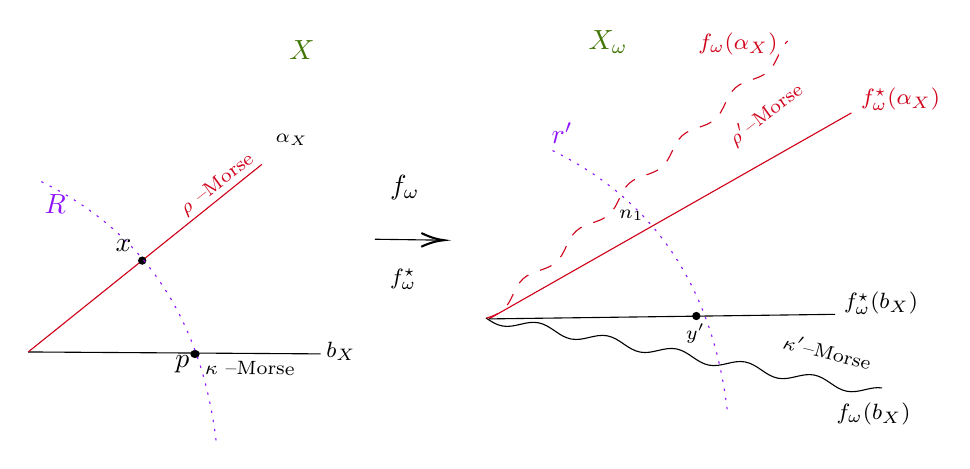
\begin{tikzpicture}[x=0.75pt,y=0.75pt,yscale=-1,xscale=1]
%uncomment if require: \path (0,300); %set diagram left start at 0, and has height of 300

%Straight Lines [id:da36450723630791704] 
\draw    (36,166.4) -- (176.91,167.33) ;
%Straight Lines [id:da5375966246891343] 
\draw [color={rgb, 255:red, 208; green, 2; blue, 27 }  ,draw opacity=1 ][fill={rgb, 255:red, 208; green, 2; blue, 27 }  ,fill opacity=1 ]   (36,166.4) -- (148.55,76.05) ;
%Shape: Wave [id:dp5760633224098543] 
\draw   (256.46,149.96) .. controls (258.96,151.67) and (261.35,153.3) .. (264.35,153.87) .. controls (267.36,154.44) and (270.15,153.79) .. (273.07,153.1) .. controls (275.99,152.42) and (278.78,151.77) .. (281.78,152.34) .. controls (284.79,152.91) and (287.18,154.54) .. (289.68,156.25) .. controls (292.17,157.96) and (294.57,159.6) .. (297.57,160.17) .. controls (300.58,160.74) and (303.37,160.09) .. (306.29,159.4) .. controls (309.2,158.71) and (311.99,158.06) .. (315,158.63) .. controls (318.01,159.2) and (320.4,160.83) .. (322.89,162.55) .. controls (325.39,164.26) and (327.78,165.89) .. (330.79,166.46) .. controls (333.79,167.03) and (336.58,166.38) .. (339.5,165.69) .. controls (342.42,165.01) and (345.21,164.35) .. (348.22,164.92) .. controls (351.22,165.49) and (353.61,167.13) .. (356.11,168.84) .. controls (358.61,170.55) and (361,172.19) .. (364,172.76) .. controls (367.01,173.33) and (369.8,172.67) .. (372.72,171.99) .. controls (375.64,171.3) and (378.43,170.65) .. (381.43,171.22) .. controls (384.44,171.79) and (386.83,173.42) .. (389.33,175.13) .. controls (391.83,176.85) and (394.22,178.48) .. (397.22,179.05) .. controls (400.23,179.62) and (403.02,178.97) .. (405.94,178.28) .. controls (408.85,177.6) and (411.65,176.94) .. (414.65,177.51) .. controls (417.66,178.08) and (420.05,179.72) .. (422.54,181.43) .. controls (425.04,183.14) and (427.43,184.78) .. (430.44,185.34) .. controls (433.44,185.91) and (436.23,185.26) .. (439.15,184.58) .. controls (441.92,183.93) and (444.56,183.31) .. (447.39,183.73) ;
%Shape: Wave [id:dp21020617893125515] 
\draw  [color={rgb, 255:red, 208; green, 2; blue, 27 }  ,draw opacity=1 ][dash pattern={on 4.5pt off 4.5pt}] (256.88,150.08) .. controls (259.73,149.13) and (262.45,148.22) .. (264.76,146.15) .. controls (267.07,144.07) and (268.33,141.39) .. (269.64,138.6) .. controls (270.96,135.8) and (272.21,133.12) .. (274.53,131.05) .. controls (276.84,128.97) and (279.56,128.06) .. (282.41,127.11) .. controls (285.27,126.16) and (287.99,125.26) .. (290.3,123.18) .. controls (292.61,121.1) and (293.87,118.43) .. (295.18,115.63) .. controls (296.49,112.83) and (297.75,110.16) .. (300.06,108.08) .. controls (302.37,106) and (305.1,105.09) .. (307.95,104.14) .. controls (310.8,103.2) and (313.53,102.29) .. (315.84,100.21) .. controls (318.15,98.13) and (319.41,95.46) .. (320.72,92.66) .. controls (322.03,89.86) and (323.29,87.19) .. (325.6,85.11) .. controls (327.91,83.03) and (330.63,82.12) .. (333.49,81.17) .. controls (336.34,80.23) and (339.06,79.32) .. (341.37,77.24) .. controls (343.68,75.16) and (344.94,72.49) .. (346.25,69.69) .. controls (347.57,66.89) and (348.82,64.22) .. (351.14,62.14) .. controls (353.45,60.06) and (356.17,59.15) .. (359.02,58.2) .. controls (361.88,57.26) and (364.6,56.35) .. (366.91,54.27) .. controls (369.22,52.19) and (370.48,49.52) .. (371.79,46.72) .. controls (373.1,43.92) and (374.36,41.25) .. (376.67,39.17) .. controls (378.98,37.09) and (381.71,36.18) .. (384.56,35.23) .. controls (387.41,34.29) and (390.14,33.38) .. (392.45,31.3) .. controls (394.76,29.22) and (396.02,26.55) .. (397.33,23.75) .. controls (398.57,21.1) and (399.76,18.56) .. (401.85,16.54) ;
%Straight Lines [id:da2014385251778429] 
\draw [color={rgb, 255:red, 208; green, 2; blue, 27 }  ,draw opacity=1 ][fill={rgb, 255:red, 208; green, 2; blue, 27 }  ,fill opacity=1 ]   (257.94,150.48) -- (432.61,51.23) ;
%Shape: Parabola [id:dp7139935681369857] 
\draw  [color={rgb, 255:red, 144; green, 19; blue, 254 }  ,draw opacity=1 ][dash pattern={on 0.84pt off 2.51pt}] (372.74,194.02) .. controls (365.5,134.42) and (337.11,92.71) .. (287.56,68.87) ;
%Shape: Free Drawing [id:dp3513930535238907] 
\draw  [line width=3] [line join = round][line cap = round] (90.92,122.39) .. controls (90.92,122.39) and (90.92,122.39) .. (90.92,122.39) ;
%Shape: Free Drawing [id:dp4625091479348489] 
\draw  [line width=3] [line join = round][line cap = round] (116.58,167.33) .. controls (116.58,167.18) and (116.28,167.33) .. (116.13,167.33) ;
%Shape: Free Drawing [id:dp28196732442037276] 
\draw  [line width=3] [line join = round][line cap = round] (357.88,149.08) .. controls (357.88,149.08) and (357.88,149.08) .. (357.88,149.08) ;
%Straight Lines [id:da3215761419383656] 
\draw    (203.02,112.09) -- (234.33,112.53) ;
\draw [shift={(236.33,112.56)}, rotate = 180.81] [color={rgb, 255:red, 0; green, 0; blue, 0 }  ][line width=0.75]    (10.93,-3.29) .. controls (6.95,-1.4) and (3.31,-0.3) .. (0,0) .. controls (3.31,0.3) and (6.95,1.4) .. (10.93,3.29)   ;
%Shape: Parabola [id:dp15036715000462286] 
\draw  [color={rgb, 255:red, 144; green, 19; blue, 254 }  ,draw opacity=1 ][dash pattern={on 0.84pt off 2.51pt}] (126.49,209) .. controls (119.25,149.41) and (90.86,107.69) .. (41.31,83.85) ;
%Straight Lines [id:da8836532210237474] 
\draw    (257.94,150.48) -- (424.73,148.27) ;

% Text Node
\draw (153.97,60.12) node [anchor=north west][inner sep=0.75pt]  [font=\scriptsize]  {$\alpha _{X}$};
% Text Node
\draw (357.67,11.61) node [anchor=north west][inner sep=0.75pt]  [font=\footnotesize,color={rgb, 255:red, 208; green, 2; blue, 27 }  ,opacity=1 ]  {$f_{\omega }( \alpha _{X})$};
% Text Node
\draw (436.04,37.93) node [anchor=north west][inner sep=0.75pt]  [font=\footnotesize,color={rgb, 255:red, 208; green, 2; blue, 27 }  ,opacity=1 ]  {$f_{\omega }^{\star }( \alpha _{X})$};
% Text Node
\draw (178.36,160.27) node [anchor=north west][inner sep=0.75pt]  [font=\footnotesize]  {$b_{X}$};
% Text Node
\draw (424.25,189.85) node [anchor=north west][inner sep=0.75pt]  [font=\footnotesize]  {$f_{\omega }( b_{X})$};
% Text Node
\draw (427.81,136.36) node [anchor=north west][inner sep=0.75pt]  [font=\footnotesize]  {$f_{\omega }^{\star }( b_{X})$};
% Text Node
\draw (76.89,111.1) node [anchor=north west][inner sep=0.75pt]    {$x$};
% Text Node
\draw (105.67,166.88) node [anchor=north west][inner sep=0.75pt]    {$p$};
% Text Node
\draw (351.54,151.44) node [anchor=north west][inner sep=0.75pt]  [font=\scriptsize]  {$y'$};
% Text Node
\draw (209.06,79.86) node [anchor=north west][inner sep=0.75pt]    {$f_{\omega }$};
% Text Node
\draw (319.45,96.66) node [anchor=north west][inner sep=0.75pt]  [font=\scriptsize]  {$n_{1}$};
% Text Node
\draw (106.26,95.3) node [anchor=north west][inner sep=0.75pt]  [font=\scriptsize,color={rgb, 255:red, 208; green, 2; blue, 27 }  ,opacity=1 ,rotate=-321.74,xslant=0.04]  {$\rho$ --Morse};
% Text Node
\draw (370.14,60.94) node [anchor=north west][inner sep=0.75pt]  [font=\scriptsize,color={rgb, 255:red, 208; green, 2; blue, 27 }  ,opacity=1 ,rotate=-321.74,xslant=0.04]  {$\rho '$--Morse};
% Text Node
\draw (120.23,169.54) node [anchor=north west][inner sep=0.75pt]  [font=\scriptsize,color={rgb, 255:red, 0; green, 0; blue, 0 }  ,opacity=1 ,rotate=-0.49,xslant=0.04]  {$\kappa$ --Morse};
% Text Node
\draw (400.49,155.66) node [anchor=north west][inner sep=0.75pt]  [font=\scriptsize,color={rgb, 255:red, 0; green, 0; blue, 0 }  ,opacity=1 ,rotate=-14.2,xslant=0.04]  {$\kappa '$--Morse};
% Text Node
\draw (286.89,54.87) node [anchor=north west][inner sep=0.75pt]  [color={rgb, 255:red, 144; green, 19; blue, 254 }  ,opacity=1 ]  {$r'$};
% Text Node
\draw (42.62,89.26) node [anchor=north west][inner sep=0.75pt]  [color={rgb, 255:red, 144; green, 19; blue, 254 }  ,opacity=1 ]  {$R$};
% Text Node
\draw (160.51,15.06) node [anchor=north west][inner sep=0.75pt]  [color={rgb, 255:red, 65; green, 117; blue, 5 }  ,opacity=1 ]  {$X$};
% Text Node
\draw (304.75,10.43) node [anchor=north west][inner sep=0.75pt]  [color={rgb, 255:red, 65; green, 117; blue, 5 }  ,opacity=1 ]  {$X_{\omega }$};
% Text Node
\draw (209.1,125.03) node [anchor=north west][inner sep=0.75pt]  [font=\footnotesize]  {$f_{\omega }^{\star }$};


\end{tikzpicture}

\caption{ $f_\omega^{\star}$ is an open map.}
\end{figure}

Now we are ready to consider any given  $\alpha \in \bfa_X$ be a $(\qq, \sQ)$--quasi-geodesic in $X$, where
\begin{enumerate}
\item $\qq, \sQ$ is such that  $\mm_{b_X}(\qq, \sQ)$ is small compared to $\rr$ with respect to $\kappa$; and
\item $f_\omega(\alpha)$ is a ray that is associated with an element in $\calU_{\kappa'}(\bfb_Y, \rr')$. 
\end{enumerate}
By the choice of $\rr'$, 
$n$ is small compared to $\rr'$. Hence, 
\[
(f_\omega^\star)(\alpha_X)=\alpha_Y|_{\rr'} \subset \calN_{\kappa'}\big(b_Y, n\big)
\] 


Pick a point $x \in \alpha_X|_{\sR}$ such that $||x||=R$ in $X$. Lets consider $d(x,b_X)$ then  $d(x,b_X)=d(x,p)$ where $p \in \Pi_{b_X}(x)$. Then if $[x,p]_\omega$ is the $\omega$-geodesic joining $x$ and $p$. Then the pre image path namely, $\beta$ satisfy, $d(\go,\beta) \leq ||x||=R \leq R \cdot \ell(\beta)$. Therefore by Proposition ~\ref{BT1}, we have
\[d(x,b_X) \leq C(R)^{-1}(d_\omega(x,b_X)  + r_o)\]

%That is $\Norm x \leq \sR$. Then $f_\omega(x) \in f_\omega( \alpha)$ also $d_\omega(\mathfrak{o},x) \leq b \cdot R+r_0$. Suppose $p$ be the point on  $f_\omega( b_X)$ such that $d_\omega(x,f_\omega(\alpha_X))=d_\omega(x,p)$. Then By lemma (?) we have $||p||_\omega \leq 2||x||_\omega \leq 2bR+r_0$ \textcolor{blue}{(\textbf{need $\rr' \geq 2bR+r_0$})} and by the choice of $\rr'$, and since $n$ is small compared to $\rr'$ we have, \[d_\omega(p,\bfb_Y)\leq 2\cdot \mm_{b_Y}(1,0)\kappa'(||x||_\omega)\] 


\begin{align*} 
d_X(x, b_X) 
&\leq C(R)^{-1}(d_\omega(x,f_\omega(b_X))  + r_o)  \\
& \leq C(R)^{-1}[d_\omega(x,\yy)+d_\omega(\yy,\yy')+d_\omega(\yy',f_\omega(b_X)] \text{\hspace{0.3cm} (where, } \yy \in \Pi_{\alpha_Y}(x), \yy' \in \Pi_{b_Y}(x))\\
& \leq C(R)^{-1}[\nn_1 \cdot \rho'(||x||_\omega)+n \cdot \kappa'(||\yy||_\omega)+\mm_{f_\omega(b_X)}(1,0) \cdot \kappa'(||\yy'||_\omega)+r_0(\omega)]\\
& \leq   C(R)^{-1}[\nn_1  +2n+4\mm_{f_\omega(b_X)}(1,0)+r_0(\omega)] \cdot \calA(||x||_\omega)
\end{align*} 
where, $\calA=\max\{\rho',\kappa'\}$.
We also have 
\[
\calA(||x||_\omega) \leq b'\cdot \calA(||x||)+r_o'  \leq (b'+r_0'(\omega)) \calA(||x||)
\]
Note that by Proposition~\ref {extension},  $C(\param)$ is a decreasing function, hence, combining the preceding inequalities, we have,

\begin{align*} 
d_X(x, b_X) & \leq C(R)^{-1}[\nn_1  +2n+4\mm_{f_\omega(b_X)}(1,0)+r_0(\omega)] \cdot \calA(||x||_\omega)\\
& \leq C(R)^{-1}[\nn_1  +2n+4\mm_{f_\omega(b_X)}(1,0)+r_0(\omega)] \cdot (b'+r_0'(\omega) \calA(||x||)\\
& \leq C(r)^{-1}[\nn_1 +2n+4\mm_{f_\omega(b_X)}(1,0)+r_0(\omega)] \cdot (b'+r_0'(\omega) \calA(||x||)\\
& \leq \nn \cdot \calA(||x||)
\end{align*}

Now, Definition ~\ref{Def:Morse} implies that 
\[
\alpha_X|_\rr \subset \calN_\kappa(b_X, \mm_{b_X}(1,0)). 
\]
Therefore, $\bfa_X \in \calU_{\kappa}(\bfb_X, \rr)$ and
\[
(f_\omega^\star)^{-1} \big(\calU_{s}(\bfb_Y, \rr')\big) \subset \calU_{s}(\bfb_X, \rr). 
\]



For the other direction, it is equivalent to saying, the $(f_\omega^\star)^{-1}$ is open. Fix a $r >0$, then we aim to show that, for any  $\calU_\kappa(\bfb_Y,r)$ the pre image $(f_\omega^\star)^{-1}(\calU_\kappa(\bfb_Y,r))$ is open in $\partial_sX$. That is, for every $\bfa_X\in (f_\omega^\star)^{-1}(\calU_\kappa(\bfb_Y,r)) $ there exists a $r'$, such that $\calU_s(\bfa_X,r') \subset (f_\omega^\star)^{-1}(\calU_\kappa(\bfb_Y,r)).$ Without loss of generality, suppose $f_\omega^\star(\bfa_X)=\bfa_Y.$ \newline
Let $R(b_Y,r,\nn, \rho')$ then choose $r'$ such that:
\begin{enumerate}
    
    \item $r' \geq \frac{R+r_1}{c}$, where $r_1, c$ are the constant from Proposition ~\ref{BT2}.
    \item $\nn'$ is small compared to $r'$.
    \end{enumerate}
Suppose, $\bfb_X \in \calU_s(\bfa_X,r')$ and $b_X$ be a geodesic representative of $\bfb_X \in \partial_sX$ and $f_\omega^\star(\bfb_X)=\bfb_Y.$ 
Suppose $a_Y$ and $b_Y$ are geodesic representatives of $\bfa_Y$ and $\bfb_Y$ in $\partial_sX_{\omega}$ respectively.  

Suppose, $y$ be a point on $a_Y$ with $||y||_\omega=R$, and let $y' \in \Pi_y(\omega(a_X))$. Now, $y''$ be the nearest point projection of $y'$ on $a_X$ in $X$. Then,
\begin{align*}
  d_\omega(y, b_Y) & \leq d_\omega(y,y')+d_\omega(y',y'')+d_\omega(y'',b_Y)\\
  &\leq m_{b_Y}(1,0) \cdot \kappa'(R)+ 2b\cdot m_{a_X}(1,0) \cdot \rho(||y'||)+ r_0(\omega)+ n_1 \cdot \rho'(||y''||_\omega)  
\end{align*}
Similarly like the previous proof there exists $\nn'$ and a sublinear function $\eta$, we have \[d_\omega(y, b_Y) \leq \nn' \cdot \eta(R)\].
\[
a_Y|_\rr \subset \calN_\kappa(b_Y, \mm_{b_Y}(1,0)). 
\]
Hence, $f_\omega^*$ is continuous. 
% \textcolor{red}{old one} ]\newline
% By Theorem~\ref{bijection}, $\Phi_\star$ defined as above gives a bijection between $\partial_sX$ 
% and $\partial_s Y$. We first show that $(\Phi_\star)^{-1}$ is continuous and will show secondly that $\Phi_\star$ is continuous. 

% Let $\calV$ be an open set in $\partial_s X$ where $\bfb_X \in \calV$. Assume without loss of generality that $\bfb_X$ is $\kappa$-Morse for some $\kappa$. 
% Then there exists a neighborhood $\calU_{\kappa}(\bfb_X, \rr) \subset \calV$. 
% Let $\bfb_Y = \Phi_\star(\bfb_X)$. By Theorem ??, there exists $\kappa'$ such that $\bfb_Y$ is $\kappa'$-Morse. We need to show that there is a constant $\rr'$ 
% such that, for every point $\bfa_Y \in \calU_\kappa'(\bfb_Y, \rr')$, we have 
% \[
% (\Phi_\star)^{-1}(\bfa_Y) = \bfa_X \in \calU_\kappa(\bfb_X, \rr).
% \]


% %\begin{figure}[h]
% %\includegraphics[width=8cm]{topologytheorem}
% %\end{figure}

% \begin{figure}[h]
% \begin{tikzpicture}[line cap=round,line join=round,>=angle 45,x=0.5cm,y=0.5cm]
% \clip(-3,-4) rectangle (17,4);
% \draw [rotate around={-63.43:(2.5,0)}] (2.5,0) ellipse (0.96cm and 0.78cm);
% \draw [rotate around={0:(2.5,0)}] (2.5,0) ellipse (1.75cm and 1.73cm);
% \draw(14.02,0) circle (1.01cm);
% \draw (-0.02,3.5) node[stuff_fill,anchor=north west] {$\mathcal V $};
% \draw (1.31,-1.31) node[stuff_fill,anchor=north west] {$ \mathcal U_{\kappa}(\mathbf b_X, \mathsf r)  $};
% \draw (12.55,-1.65) node[stuff_fill,anchor=north west] {$ \mathcal U_{\kappa}(\mathbf b_Y, \mathsf r') $};
% \begin{scriptsize}
% \fill [color=black] (2.73,-0.27) circle (1.5pt) node[anchor=north] {$\mathbf b_X$} ;
% \fill [color=black] (2.13,0.27) circle (1.5pt)  node[anchor=south] {$\mathbf a_X$} ;
% \fill [color=black] (14.05,-0.16) circle (1.5pt)  node[anchor=north] {$\mathbf b_Y$} ;
% \fill [color=black] (15.25,0.16) circle (1.5pt)  node[anchor=north] {$\mathbf a_Y$} ;
% \end{scriptsize}
% \draw [color = black,->] (7,0) -- (11,0);
% \draw [color = black] (9,-0.5) node[anchor=center] {$\Phi_\star$};
% \end{tikzpicture}
% \caption{$\Phi_\star$ is a homeomorphism.}
% \end{figure}

% First, we find the upper bound for the constants $\qq', \sQ'$ where
% \begin{enumerate}
% \item $\mm_{b_X}(\qq, \sQ)$ is small compared to $\rr$ (with respect to the function $\kappa$), and
% \item If $\zeta$ is a $(\qq, \sQ)$--quasi-geodesic ray in $X$ then $\Phi \zeta$ is in a $n \cdot \kappa'$-neighbourhood of a $\kappa'$ Morse geodesic ray (Lemma 3.6).
% \end{enumerate}
% We obtain this by using Theorem~\ref{tracking} and  let $\qq'=k \qq$ and $\sQ' = \qq K + \kappa'(\qq r)$ be constants (depending on $\qq, \sQ, L$ and $\sK$).
% %%%%%%%%%%%%%%%%%%%%%%%%%

% Next, let $b_Y$ be the representative geodesic ray in $\bfb_Y$ and let $\mm_{b_X} \cdot \kappa$ and 
% $\mm_{b_Y} \cdot \kappa$ be their sublinearly Morse gauges respectively. 
% By Lemma~\ref{L:symmetry}, there is
% a constant $\nn_1$ depending on $L, \kappa, \kappa'$ and $\mm_{b_Y} \cap B(\go, r)$ such that 
% \[
% \Phi b_X \subset \calN_\kappa(b_Y, \nn_1). 
% \]
% Next, we let 
% \[
% \nn = \frac{1}{c(r)} \big( n + \nn_1\big) (\frac{1}{c(r)} + 1) + 1
% \]
% and let $\sR = \sR(b_X, \rr, \nn, \kappa')$ as in Definition~\ref{defn:Morse} and 
% choose $\rr'$ such that:
% \begin{enumerate}
% \item $\rr' \geq c(\sR) + \kappa(r)$, and
% \item $n$ is small 
% compare to $\rr'$.
% \end{enumerate}

% Now we are ready to consider any given  $\alpha \in \bfa_X$ be a $(\qq, \sQ)$--quasi-geodesic in $X$, where
% \begin{enumerate}
% \item $\qq, \sQ$ is such that  $\mm_{b_X}(\qq, \sQ)$ is small compared to $\rr$ with respect to $\kappa$; and
% \item $\Phi \alpha$ is a ray that is in $\calU_{\kappa'}(\bfb_Y, \rr')$. 
% \end{enumerate}
% By the choice of $\rr'$, 
% $n$ is small compared to $\rr'$. Hence, 
% \[
% \Phi \alpha|_{\rr'} \subset \calN_\kappa'\big(b_Y, n\big)
% \] 
% Pick a point $x \in \alpha_X|_{\sR}$. Then $\Phi x \in \Phi \alpha|_{\rr'}$ and we have 

% \begin{align*} 
% d_X(x, b_X) &\leq (c(R))^{-1}(d_Y(\Phi(x), \Phi b_X) + r_0(\omega)\\
% & \leq (c(R))^{-1} \Big(d_Y(\Phi(x), b_Y) + \nn_1 \cdot \kappa'(\Phi x) \Big)+ r_0(\omega) \\
% & \leq (c(R))^{-1} \big( n+ \nn_1\big) \cdot \kappa'(\Phi x) r_0(\omega) +\\
% & \leq(c(R))^{-1}\big( n + \nn_1\big) \cdot \kappa'(\Phi x)  +r_0(\omega)
% \end{align*} 
% We also have 
% \[
% \kappa'(\Phi x) \leq  (c(R))^{-1}\kappa'(x)  \leq ( (c(R))^{-1}+ 1) \kappa'(x)
% \]
% Note that $c(\param)$ is decreasing (Lemma??), thus  $(c(\param))^{-1}$ is an increasing function. Combine the preceding inequalities we have
% \begin{align*} 
% d_X(x, b_X) &\leq (c(R))^{-1}\big( n + \nn_1\big) \cdot  ( (c(R))^{-1} + 1) \kappa'(x) + r_0(\omega)\\
%                     &\leq \Big ( (c(R))^{-1} \big( n + \nn_1\big) ( (c(R))^{-1} + 1) +1 \Big) \kappa'(x)\\
%                     &\leq \Big (c(r)^{-1} \big( n + \nn_1\big) ((c(r))^{-1} + 1) +1 \Big) \kappa'(x)\\
%                     &= \nn\kappa'(x).
% \end{align*}
% imply that 
% \[
% \alpha|_{\sR} \subset \calN_\kappa(b_X, \nn). 
% \]
% Now, Definition~\ref{defn:Morse} implies that 
% \[
% \alpha|_\rr \subset \calN_\kappa(b_X, \mm_{b_X}). 
% \]
% Therefore, $\bfa_X \in \calU_{\kappa}(\bfb_X, \rr)$ and
% \[
% (\Phi_\star)^{-1} \calU_{\kappa'}(\bfb_Y, \rr') \subset \calU_{\kappa'}(\bfb_X, \rr). 
% \]
% But $ \calU_{\kappa}(\bfb_Y, \rr') $ contains an open neighbourhood of $\bfb_Y$, therefore, 
% $\bfb_Y$ is in the interior of $\Phi \calV$. This finishes the proof in one direction. The opposite direction is identitcal withe $c(R)$ replaced by $b$. 
\end{proof} 

Lastly, we would like to quickly observe that since sublinearly Morse boundaries are visibility spaces \cite[Theorem C]{DZ}, for any two directions $\alpha, \beta \in \pka X$, there exists a bi-infinite geodesic line in $X_\omega$ that converges to them. This is also an observation analogous to \cite[Theorem 1.13]{BM2}.
\begin{corollary}
    Let $X$ be an infinite graph with uniformly bounded degree. For almost every $\omega$, consider any two distinct element in $\pka X$,  there exists a bi-infinite geodesic line in $X_{\omega}$  that converges to these two directions in $\pka X_\omega$.
\end{corollary}
\begin{proof}

Fix distinct $\xi_1,\xi_2\in \partial_s X$. For almost every $\omega$, the map $f_\omega^\star:\partial_s X\to \partial_s X_\omega$ is a homeomorphism, hence
$f_\omega^\star(\xi_1)\neq f_\omega^\star(\xi_2)$. Choose $\kappa$-Morse
quasi-geodesic rays $\alpha_1^\omega,\alpha_2^\omega$ in $X_\omega$, both based
at $\go$, representing $f_\omega^\star(\xi_1)$ and $f_\omega^\star(\xi_2)$,
respectively. Since these boundary points are distinct, the rays
$\alpha_1^\omega$ and $\alpha_2^\omega$ do not $\kappa$-fellow travel. By the
Theorem 2.13 in \cite{DZ}, there exists a bi-infinite geodesic line
$\beta_\omega:\mathbb{R}\to X_\omega$ whose two half-rays are $\kappa$-equivalent
to $\alpha_1^\omega$ and $\alpha_2^\omega$. Hence the two ends of $\beta_\omega$
represent $f_\omega^\star(\xi_1)$ and $f_\omega^\star(\xi_2)$.

\end{proof}



%\bibliography{Citations}{}
\bibliographystyle{alpha}
\begin{thebibliography}{AKB12}

% \bibitem[ACGH17]{Hume}
% G. Arzhantseva, C. Cashen, D. Gruber, and D. Hume,
% \newblock{ Characterizations of Morse quasi-geodesics via superlinear divergence and sublinear contraction},
% \newblock{ \em Documenta Mathematica} 22 (2017), 1193--1224.
\bibitem[ADT17]{ADT}
Tarik Aougab, Matthew Durham and Samuel Taylor.
\newblock{Pulling back stability with applications to $Out(F_n)$}. 
\newblock{\em Journal of the London Mathematical Society}, vol. 96, iss. 3 (2017)

%  \bibitem[Bal95]{Ballman} 
%  W. Ballmann.
%   \newblock{Lectures on Spaces of Nonpositive Curvature} ,
%    \newblock{\em DMV Seminar} Volume 25 Birkhauser Verlag, Basel, 1995

%  \bibitem[BB08]{BB08} 
% W. Ballmann and S. Buyalo. 
% \newblock{\em  Periodic rank one geodesics in Hadamard spaces}.
% \newblock{\em Geometric and probabilistic structures in dynamics}, volume 469 of Contemp. Math., pages 19--27. Amer. Math. Soc., Providence, RI, 2008.

% \bibitem[BF09]{BF09}
% Mladen Bestvina and Koji Fujiwara.
% \newblock{ A Characterization of Higher Rank Symmetric Spaces Via Bounded Cohomology},
% \newblock{\em Geometric and Functional Analysis} volume 19, pages 11--40 (2009)


% \bibitem[BGH16]{BGH} 
% H. Baik, I. Gekhtman, and U. \Ham,
% \newblock {The smallest positive eigenvalue of fibered hyperbolic 3-manifolds},
% \newblock {\em Proceedings of the London Mathematical Society}, Volume 120, Issue 5, 704--741.




\bibitem[BH09]{BH1}
Martin~R. Bridson and Andr\'{e} H\"{a}fliger.
\newblock {\em Metric Spaces of Non-Positive Curvature},
\newblock {Springer}, 2009.

\bibitem[BJQ25]{BJQ}
Dominic Bair, Sagnik Jana and Yulan Qing
\newblock {\em First-passage percolation, non-positive curvature, and radial maps},
\newblock {preprint}, 2025.

% \bibitem[BK02]{BK02}
% Benakli, Nadia and Kapovich, Ilya.
% \newblock {\em Boundaries of hyperbolic groups},
% \newblock {\em arXiv preprint math/0202286}


% \bibitem[BM96]{Burger-Mozes} 
% Marc Burger and Shahar Mozes.
% \newblock{CAT(-1)-Spaces, Divergence Groups and their Commensurators},
% \newblock{\em Journal of the American Mathematical Society} Vol. 9, No. 1 (Jan., 1996), pp. 57--93.

\bibitem[BM22]{BM1} 
Riddhipratim Basu and Mahan Mj 
\newblock{First passage percolation on hyperbolic groups.}
\newblock{\em Advances in Mathematics}
Volume 408, Part A, 29 October 2022, 108599.

\bibitem[BM24]{BM2} 
Riddhipratim Basu and Mahan Mj
\newblock{Geodesic Trees and Exceptional Directions in FPP on Hyperbolic Groups}
\newblock{\em preprint.}arXiv:2412.03067 



\bibitem[BT17]{BT17} 
Itai Benjamini and Romain Tessera. 
\newblock{First passage percolation on a hyperbolic graph
admits bi-infinite geodesics.}
\newblock{\em Electron. Commun. Probab.}, 22:Paper No. 14, 8, 2017.

\bibitem[BZ12]{BZ12}
Itai Benjamini and Ofer Zeitouni. 
\newblock{Tightness of fluctuations of first passage percolation
on some large graphs. }
\newblock{\em In Geometric aspects of functional analysis}, volume 2050 of
Lecture Notes in Math., pages 127–132. Springer, Heidelberg, 2012.


 \bibitem[Cas16]{cashen}
C. Cashen,
\newblock{ Quasi-isometries need not induce homeomorphisms of contracting boundaries with the Gromov product topology},
\newblock{\em Analysis and Geometry in Metric Spaces} 4 (2016), no. 1, 278--281.
% \bibitem[CCM19]{CCM19}
% Ruth Charney, Matthew Cordes, Devin Murray,
% \newblock{Quasi-Mobius Homeomorphisms of Morse boundaries},
% \newblock{\em Bulletins of the London Mathematical Society} 24 March 2019

% \bibitem[CC20]{caglarclay}
% C. Uyanik and M. Clay
% \newblock{Atoroidal dynamics of subgroups of Out(Fn)},
% \newblock{\em J. London Math. Soc.}, 102 (2020), 818-845. [

\bibitem[Choi22]{Choi}
Inhyeok Choi.
\newblock{Limit laws on Outer space, Teichm\"uller space, and \CAT spaces},
\newblock{\em arXiv:2207.06597}

% \bibitem[CK00]{CK00}
% C. B. Croke and B. Kleiner.
% \newblock{\em Spaces with nonpositive curvature and their ideal boundaries},
% \newblock{\em Topology 39 (2000), no. 3, 549--556.}


% \bibitem[CLM12]{Leininger}
% C. Leininger, M. Clay and J. Mangahas.
% \newblock{ The geometry of right angled Artin subgroups of mapping class groups},
% \newblock{ \em Groups Geom. Dyn.} 6 (2012), no. 2, 249--278.

% \bibitem[CM19]{cashenmackay}
% C. Cashen and J. Mackay,
% \newblock{ A metrizable topology on the contracting boundary of a group},
% \newblock{\em Transactions of the American Mathematical Society} 372 (2019), no. 3, 1555--1600.



\bibitem[Cou22]{Coulon}
R\'emi Coulon.
\newblock {Patterson-Sullivan theory for groups with a strongly contracting element}
\newblock {\em arxiv:2206.07361}

% \bibitem[Cou23]{Cou23}
% R\'emi Coulon.
% \newblock{Ergodicity of the geodesic flow for groups with a contracting element}
% \newblock{\em	arXiv:2303.01390}




\bibitem[Cor18]{Cordes}
M. Cordes,
\newblock {Morse boundaries of proper geodesic spaces},
\newblock {\em Groups Geom. Dyn. 11 (2017), no. 4, 1281--1306}.


% \bibitem[CS11]{CS11}
% P.-E. Caprace and M. Sageev. 
% \newblock {Rank rigidity for CAT(0) cube complexes.}
% \newblock {\em Geom. Funct. Anal.}, 21(4):851--891, 2011.

\bibitem[CS15]{CS}
R. Charney and H. Sultan,
\newblock {Contracting boundaries of \CAT},
\newblock {\em J. Topology} 8 (2015), no. 1, 93--117.

% \bibitem[CT21]{CT21}
%  Sean Cleary and Ariadna Fossas Tenas,
% \newblock,
% \newblock{\em M\"unster J. of Math.} 14 (2021), 485–496.

\bibitem[DMS09]{DMS}
Cornelia Drutu, Shahar Mozes, Mark Sapir.
\newblock {Divergence in lattices in semisimple Lie groups}
and graphs of groups.
\newblock {\em Transaction of The American Mathematical Society}
Volume 362, Number 5, May 2010, Pages 2451--2505.

\bibitem[DV15]{DV15}
J. Dydak and \v{Z} Virk.
\newblock{Inducing maps between Gromov boundaries}
\newblock{\em Mediterranean Journal of Mathematics} 
Volume 13, November 2015, Pages 2733--2752


\bibitem[DZ22]{DZ}
Matthew Durham and Abdul Zalloum.
The geometry of genericity in mapping class groups and Teichm\"uller space via CAT(0) cube complexes. 
\newblock{\em arXiv:2207.06516}

% \bibitem[FLP12]{FLP}
%  Albert Fathi, Fran\c{c}ois Laudenbach, and Valentin Po\'{e}naru.
% \newblock{ Thurston's Work on Surfaces, Translated from the 1979 French original by Djun M. Kim and Dan Margalit }
% \newblock{\em Princeton University Press, Princeton, NJ} 2012

% \bibitem[Fur02]{Furman} 
% Alex Furman.
% \newblock{Random walks on groups and random transformations,}
% \newblock{\em Handbook of
% dynamical systems} Vol. 1A, 931--1014, North-Holland, Amsterdam, 2002.

% \bibitem[Fur73]{Furstenberg}
% Harry Furstenberg.
% \newblock{Boundary theory and stochastic processes on homogeneous spaces.}
% \newblock{\em In Harmonic analysis on homogeneous spaces} (Proc.
% Sympos. Pure Math., Vol. XXVI, Williams Coll., Williamstown, Mass.,
% 1972), 1973.

% \bibitem[Ger12]{Victor}
% Victor Gerasimov,
% \newblock{Floyd maps for relatively hyperbolic groups}
% \newblock{\em Geometric and Functional Analysis}, Volume 22, pages 1361–1399, (2012)

% \bibitem[GGPY21]{GGPY} 
% Ilya Gekhtman, Victor Gerasimov, Leonid Potyagailo, and Wenyuan Yang.
% \newblock{Martin boundary covers Floyd boundary} ,
% \newblock{\em Inventiones Mathematicae} no 223, 759--809(2021).
% % \bibitem[GM91]{GM}
% % Frederick P. Gardiner an Howard Masur.
% % \newblock  {Extremal length geometry of \Teich space}, 
% % \newblock {\em Complex Variables Theory Appl.}, 16 (1991), no. 2-3, 209--237.



\bibitem[Gou22]{Gou22}
Sebastien Gou\"ezel. 
\newblock{Exponential bounds for random walks on hyperbolic spaces without moment conditions.}
\newblock{\em Tunis. J. Math.}, 4(4):635--671, 2022.

\bibitem[GQR22]{GQR22} 
I.~Gekhtman, Y.~Qing, K.~Rafi
\newblock{Genericity of sublinearly Morse directions in CAT(0) spaces and the Teichmüller space}. 
\newblock{\em Mathematische Zeitschrift}, Vol 311 2022.

\bibitem[Gro87]{gromov}
M. Gromov,
\newblock{Hyperbolic groups},
\newblock{ \em In Gersten, Steve M. (ed.). Essays in group theory}, Mathematical Sciences Research 
  Institute Publications. 8. New York: Springer. 75--263. 



% \bibitem[HM79]{Hubbard-Masur}
% John Hubbard and Howard Masur. 
% \newblock {Quadratic differentials and foliations},
% \newblock {\em Acta Mathematica} volume 142, pages 221--274 (1979).


% \bibitem[Hub06]{Hubbard}
% J.Hubbard.
% \newblock {Teichm\"uller theory and applications to geometry, topology and dynamics},
%  \newblock {\em Matric Edition, Ithaca}
% 2006. 
% \bibitem[HW08]{wise}
% D.Wise and F.Haglund.
% \newblock{Special Cube Complexes,}
% \newblock{\em Geom. Funct. Anal.} (2008) 17 no.5, 1551--1620.

\bibitem[HW65]{HW65}
J. M. Hammersley and D. J. A. Welsh. 
\newblock{First-passage percolation, subadditive processes,
stochastic networks, and generalized renewal theory. }
\newblock{\em In Proc. Internat. Res. Semin.},
First passage percolation on hyperbolic groups 53
Statist. Lab., Univ. California, Berkeley, Calif, pages 61–110. Springer-Verlag, New
York, 1965.



% \bibitem[IZ24]{IZ24}
% M. Incerti-Medici and A. Zalloum,
% \newblock {Sublinearly Morse boundaries from the view point of combinatorics }
% \newblock {\em Forum Mathematicum}, to appear.

\bibitem[JQ25]{JanaQing1}
Sagnik Jana, Yulan Qing.
\newblock{Sublinear geodesics in first passage percolations}
\newblock{\em preprint}  arXiv:2507.07859

% \bibitem[KB02]{kapovich2002boundaries}
% I. Kapovich and N. Benakil.
% \newblock{In R. Gillman et al., editors,}
% \newblock{\em Combinatorial and Geometric Group Theory,}
% \newblock{volume 296 of}
% \newblock{\em Contemporary Mathematics,}
% \newblock{pages 39-94. American Mathematical Society, Providence, RI, 2002.}
\bibitem[Kes84]{Kesten}
H. Kesten. 
\newblock{\em Aspects of first passage percolation. }
\newblock{\em École d’Été de probabilité de Saint-Flour XIV}
- 1984, Lecture Notes in Math., 1180, Springer, Berlin, (1986) 125–264.

% \bibitem[KM99]{KarlssonMargulis}  
% A. Karlsson and G. Margulis.
% \newblock{A multiplicative ergodic theorem and nonpositively curved spaces,}
% \newblock{\em Comm. Math. Phys.} 208 (1999) 107--123.


% \bibitem[KM96]{Kaimanovich-Masur}
% Vadim A. Kaimanovich and Howard A. Masur.
% \newblock{The Poisson boundary of the mapping class group}, 
% \newblock{\em Invent. Math. }125 (1996), no. 2, 221--264.

% \bibitem[Kai00]{KaiHyp}
% Vadim A. Kaimanovich.
%   \newblock{The Poisson formula for groups with hyperbolic properties,}
%   \newblock{\em Ann. of Math. }(2) 152 (2000), no. 3, 659--692.

% \bibitem[Kar03]{Karlsson}
% Anders Karlsson,
% \newblock{Free Subgroups of Groups with Nontrivial Floyd Boundary},
% \newblock{\em Communications in Algebra} Vol. 31, No. 11, pp. 5361--5376, 2003.



%\bibitem{KarlssonMargulis}  
%A. Karlsson, G. Margulis, A multiplicative ergodic theorem and nonpositively curved spaces. Commun. Math. Phys. 208 (1999), 107-123.

% \bibitem[Kla]{Klarreich} 
% E. Klarreich.
% \newblock{the boundary at Infinity of the Curve Complex and the Relative Teichm\"uller
% Space },
% \newblock{\em Preprint} arxiv:1803.10339

% \bibitem[KL08]{Kent-Leininger}
% R. P. Kent, and C. J. Leininger.
% \newblock {Shadows of mapping class groups: capturing convex cocompactness},
% \newblock {\em Geom. Funct. Anal.} 18 (2008).



% \bibitem[Lea13]{Lea}
% Ian J. Leary,
% \newblock { A metric Kan–Thurston theorem},
%  \newblock {\em Journal of Topology}, Volume 6, Issue 1, 2013, 1--284.



% \bibitem[LeB]{LeBars}
% Corentin Le Bars.
% \newblock {Random walks and rank-1 isometries on \CAT spaces.}
% \newblock {\em  arxiv:2205.07594}

% \bibitem[Len08]{Lenzhen}
% A.Lenzhen.
% \newblock {Teichm\"uller geodesics that do not have a limit in $\mathcal{PMF}$},
% \newblock {\em Geom.Topol. }12(2008),no.1,177--197.


%
%\bibitem[ACGH17]{sub}
%Arzhantseva, Cashen, Gruber and Hume
%\newblock {Characterizations of mores quasi-geodesics via superlinear divergence and sublinear contraction}
%\newblock {\em Documenta Mathematica} (31 August 2017) 
%
\bibitem[Cor18]{Mores}
Matthew Cordes
\newblock {morse boundaries of proper geodesic spaces.}
\newblock {\em Groups, Geometry, and Dynamics.} 11 (2017), no. 4, 1281-1306.

%\bibitem[Cha07]{intro}
%Ruth Charney
%\newblock{An introduction to right-angled Artin groups.}
%\newblock {\em Geometriae Dedicata.} Volume 125(2007), Issue 1, pp 141-158 
%
%\bibitem[BHS17]{factorsystem}
%J. Behrstock, M. Hagen and A. Sisto
%\newblock{Hierarchically hyperbolic spaces I: curve complexes for cubical groups.} 
%\newblock{\em Geometry \& Topology}  vol 21, 1731-1804, 2017.
%
%\bibitem[BC12]{ssh}
%J. Behrstock and R. Charney
%\newblock{Divergence and quasimorphisms of right-angled Artin groups.} 
%\newblock{\em Mathematische Annalen} vol. 352, 339--356, 2012.



% \bibitem[Lin17]{Link} 
% Gabriele Link.
%   \newblock{ Hopf-Tsuji-Sullivan dichotomy for quotients of Hadamard spaces with a rank-1 isometry},
%     \newblock{\em Discrete and Continuous Dynamical Systems} 38(11) (2017).
    
% \bibitem[Lin20]{Link2} 
% Gabriele Link.
%   \newblock{ Equidistribution and counting of orbit points for discrete rank-1 isometry groups of Hadamard spaces,}
%   \newblock{ \em Tunisian Journal of Mathematics} 2(4) (2020) 791--839.

% \bibitem[Mas80]{MasurUE} 
% Howard Masur.
% \newblock{Uniquely ergodic quadratic dierentials},
% \newblock{\em Comment. Math. Helvetici} Vol. 55 (1980) 255--266. 

% \bibitem[LLR18]{LLR}
% Christopher Leininger, Anna Lenzhen and Kasra Rafi.
% \newblock { Limit sets of Teichm\"uller geodesics with minimal non-uniquely ergodic vertical foliation},
% \newblock {\em Journal f\"ur die reine und angewandte Mathematik} 737 (2018), 1--32.

% \bibitem[L\"oh18]{Clara}
% Clara L\"oh,
% \newblock{Geometric Group Theory An Introduction}, 
% \newblock{\em   Universitext, Springer, } ISBN 978-3-319-72253-5, 2017. 


% \bibitem[Liu19]{liu2021dynamics}
% Q. Liu,
% \newblock{Dynamics on the Morse boundary},
% \newblock{\em  Geometriae Dedicata}, 2019.

% \bibitem[Min96]{Minsky}
% Y. Minsky.
% \newblock {Quasi-projections in Teichm\"uller space},
% \newblock{\em J. Reine Angew. Math.} 473 (1996), 121--136.

% \bibitem[MQZ22]{MQZ20}
% Devin Murray, Yulan Qing, Abdul Zalloum.
% \newblock{Sublinearly Morse Geodesics in CAT(0) Spaces: Lower Divergence and Hyperplane Characterization}
% \newblock{\em Algebraic \& Geometric Topology} 22 (2022) 1337-1374. 


% \bibitem[NQ24]{NQ}
% Hoang Thanh Nguyen and Yulan Qing.
% \newblock{Sublinearly Morse Boundary of CAT(0) admissible groups}
% \newblock{\em Journal of Group Theory},to appear.


% \bibitem[PH22]{Penner}
% R. C. Penner, with J. L. Harer.
% \newblock{Combinatorics of Train Tracks},
% \newblock{\em Annals of Mathematics Studies 1922} Princeton University Press.

 \bibitem[PQ24]{PQ24}
Gabriel Pallier and Yulan Qing,
\newblock{Sublinear biLipschitz equivalence and sublinearly Morse boundaries},
\newblock{\em Journal of the London Mathematical Society}110 (2).
 



\bibitem[QRT22]{QRT1}
Yulan Qing, Kasra Rafi and Giulio Tiozzo 
\newblock {Sublinearly Morse boundaries I:  \CAT spaces},
\newblock {\em Advances in Mathematics} 404 (2022) 108442. 


\bibitem[QRT23]{QRT2} 
Yulan Qing, Kasra Rafi and Giulio Tiozzo. 
\newblock {Sublinearly Morse boundaries II:  Proper geodesic spaces,}
\newblock{\em Geometry \& Topology} 28(4) (2024) 1829--1889.

\bibitem[QR24]{QR24} 
Yulan Qing, Kasra Rafi. 
\newblock {The quasi-redirecting boundary}
\newblock{\em arxiv:2406.16794}.

\bibitem[QY24]{QY24}
Yulan Qing and Wenyuan Yang.
\newblock {\em Genericity of sublinearly Morse directions in general metric spaces}.
\newblock{arxiv:2404.18762}.



\bibitem[QZ24]{QZ}
Yulan Qing and Abdul Zalloum.
\newblock {Topological properties of sublinearly Morse boundaries of CAT(0) groups.}
\newblock { Pacific Journal of Mathematics}, to appear.


% \bibitem[Ric17]{Ricks} 
% R. Ricks.
%   \newblock{Flat strips, Bowen-Margulis measures, and mixing of the geodesic flow for rank-1 \CAT spaces, }
%   \newblock{\em Ergodic Theory Dynam. Systems,} no. 3, 37 (2017), 939--970.

%\bibitem[Thu86]{FLP}
%W. Thurston
%\newblock{ Geometry and topology of 3-manifolds}
%\newblock{\em Princeton University Lecture Notes} 1986, http://
%www.msri.org/publications/books/gt3m.

% \bibitem[Tio15]{Tiozzo}
% Giulio Tiozzo.
% \newblock{Sublinear deviation between geodesics and sample paths},
% \newblock{\em Duke Math. J.}  164 (2015), no. 3, 511--539.


% \bibitem[Thu88]{Thurstoncircle}
% W. P. Thurston, 
% \newblock{On the geometry and dynamics of diffeomorphisms of surfaces},
% \newblock{\em Bull. Amer. Math. Soc.} (N.S.) 19 (1988), no. 2, 417–431.

\bibitem[Wen25]{rouwen25}
Rou Wen,
\newblock{Sublinearly morseness in higher rank symmetric spaces}
\newblock{\em arXiv:2504.12448} 


\bibitem[Yan22]{wenyuan}
Wenyuan Yang.
\newblock {Conformal dynamics at infinity for groups with contracting elements},
\newblock {\em arXiv:2208.04861.} 

 
% \bibitem[Zal22]{Z}
%  Abdul Zalloum.
% \newblock{Convergence of sublinearly contracting horospheres}
% \newblock{\em Geometriae Dedicata} 216, 35 (2022).

 \end{thebibliography}
\end{document}
